\section[Developer survey]{Developer survey}
\label{sec:evaluation:developer-survey}

%\subsection{User Study}
%\label{sec:evaluation:developer-survey}

The developer-oriented user study was conducted to assess the simplicity\index{Simplicity} of file-based repository\index{Repository} implementations and the easy of interaction with such implementations.

\subsection{Target population}
\label{sec:evaluation:developer-survey:target-population}

The survey participants were recruited from a total of \num{34} Computer Science Honours (CSC4000) students, enrolled for the \gls{www}\index{WWW} elective course module at the University of Cape Town.

The \gls{www}\index{WWW} module had a mandatory practical assignment, accounting for \SI{20}{\percent} of the overall assessment, in which the students were required to build generic Web\index{Web} applications, in groups, using the file-based repository store described in Section~\ref{sec:case-studies:bleek-and-lloyd}. Screenshots of the online questionnaire are in the Appendix section\footnote{Please see Appendix~\ref{ch:appendex-b:developer-survey:questionnaire-design} for details}, and show the assignment question. A request for survey participation was emailed to the class mailing list after the assignment due date, in which \num{26} out of the \num{34} students responded, as shown in Table~\ref{tab:experimentation:survey:target-population}

\tablespacing
%%%%%\begin{longtable}{p{0.15\linewidth} p{0.035\linewidth}
%%%%%p{0.035\linewidth} p{0.035\linewidth} p{0.035\linewidth} p{0.035\linewidth}
%%%%%p{0.035\linewidth} p{0.035\linewidth} p{0.035\linewidth} p{0.035\linewidth}
%%%%%p{0.035\linewidth} p{0.035\linewidth} p {0.035\linewidth}}
\begin{longtable}{
>{\arraybackslash}p{0.18\linewidth}|
>{\centering\arraybackslash}p{0.035\linewidth}|
>{\centering\arraybackslash}p{0.035\linewidth}|
>{\centering\arraybackslash}p{0.035\linewidth}|
>{\centering\arraybackslash}p{0.035\linewidth}|
>{\centering\arraybackslash}p{0.035\linewidth}|
>{\centering\arraybackslash}p{0.035\linewidth}|
>{\centering\arraybackslash}p{0.035\linewidth}|
>{\centering\arraybackslash}p{0.035\linewidth}|
>{\centering\arraybackslash}p{0.035\linewidth}|
>{\centering\arraybackslash}p{0.035\linewidth}|
>{\centering\arraybackslash}p{0.035\linewidth}|
>{\centering\arraybackslash}p{0.035\linewidth}}


\caption{Developer survey target population}
\label{tab:experimentation:survey:target-population}\\
 %%%%%\toprule
 %%%%%\cline{2-13}
 %%{} & \multicolumn{11}{c}{\textbf{Practical Assignment Group}}\\
 %%\midrule
 \textbf{} & 
 \multicolumn{1}{c|}{\begin{sideways}\textbf{Group 1}\end{sideways}} &
 \multicolumn{1}{c|}{\begin{sideways}\textbf{Group 2}\end{sideways}} &
 \multicolumn{1}{c|}{\begin{sideways}\textbf{Group 3}\end{sideways}} &
 \multicolumn{1}{c|}{\begin{sideways}\textbf{Group 4}\end{sideways}} &
 \multicolumn{1}{c|}{\begin{sideways}\textbf{Group 5}\end{sideways}} &
 \multicolumn{1}{c|}{\begin{sideways}\textbf{Group 6}\end{sideways}} &
 \multicolumn{1}{c|}{\begin{sideways}\textbf{Group 7}\end{sideways}} &
 \multicolumn{1}{c|}{\begin{sideways}\textbf{Group 8}\end{sideways}} &
 \multicolumn{1}{c|}{\begin{sideways}\textbf{Group 9}\end{sideways}} &
 \multicolumn{1}{c|}{\begin{sideways}\textbf{Group 10}\end{sideways}} &
 \multicolumn{1}{c|}{\begin{sideways}\textbf{Group 11}\end{sideways}} &
 \multicolumn{1}{c}{\begin{sideways}\textbf{Group 12}\end{sideways}}\\
 %%%%%\midrule
 \cline{1-13}
 \endfirsthead
 
 \caption[]{(continued)}\\
 %%%%%\toprule
 %%%%%\cline{2-13}
 %%{} & \multicolumn{12}{c}{\textbf{Programming Group}}\\
 %%\midrule
 \textbf{} & 
 \multicolumn{1}{c|}{\begin{sideways}\textbf{Group 1}\end{sideways}} &
 \multicolumn{1}{c|}{\begin{sideways}\textbf{Group 2}\end{sideways}} &
 \multicolumn{1}{c|}{\begin{sideways}\textbf{Group 3}\end{sideways}} &
 \multicolumn{1}{c|}{\begin{sideways}\textbf{Group 4}\end{sideways}} &
 \multicolumn{1}{c|}{\begin{sideways}\textbf{Group 5}\end{sideways}} &
 \multicolumn{1}{c|}{\begin{sideways}\textbf{Group 6}\end{sideways}} &
 \multicolumn{1}{c|}{\begin{sideways}\textbf{Group 7}\end{sideways}} &
 \multicolumn{1}{c|}{\begin{sideways}\textbf{Group 8}\end{sideways}} &
 \multicolumn{1}{c|}{\begin{sideways}\textbf{Group 9}\end{sideways}} &
 \multicolumn{1}{c|}{\begin{sideways}\textbf{Group 10}\end{sideways}} &
 \multicolumn{1}{c|}{\begin{sideways}\textbf{Group 11}\end{sideways}} &
 \multicolumn{1}{c}{\begin{sideways}\textbf{Group 12}\end{sideways}} \\
 %%%%%\midrule
 \cline{1-13}
 \endhead
 
 % Page footer
 %%%%%\midrule
 \cline{1-13}
 \multicolumn{9}{r}{(Continued on next page)} \\
 \endfoot
 
 % Last page footer
 %%%%%\bottomrule
 \endlastfoot
 
 %   &
 \textbf{Candidates}& {3}& {3}& {3}& {3}& {3}& {2}& {3}& {3}& {3}& {3}& {3}& {2}\\
 
 \cline{1-13}
 %\cmidrule[0.1pt](l{0.5em}r{0.5em}){1-13}
 
 %  &
 \textbf{Respondents}& {3}& {3}& {1}& {2}& {2}& {3}& {3}& {1}& {2}& {2}& {1}& {2}\\
 
 %\cmidrule[0.1pt](l{0.5em}r{0.5em}){1-13}
 
\end{longtable}

\bodyspacing

\subsection{Data collection}
\label{sec:evaluation:developer-survey:data-collection}

A post-experiment survey was conducted in the form of an online questionnaire\footnote{Please see to Appendix~\ref{ch:appendex-b:developer-survey:questionnaire-design} for details}, designed using LimeSurvey\footnote{\url{http://www.limesurvey.org}}\index{LimeSurvey}. The questionnaire was aimed at eliciting participants' experience in working with a file-based collection.

\begin{figure}
 \centering
 \framebox[\textwidth]{
 % Created by tikzDevice version 0.6.2-92-0ad2792 on 2013-04-07 18:12:23
% !TEX encoding = UTF-8 Unicode
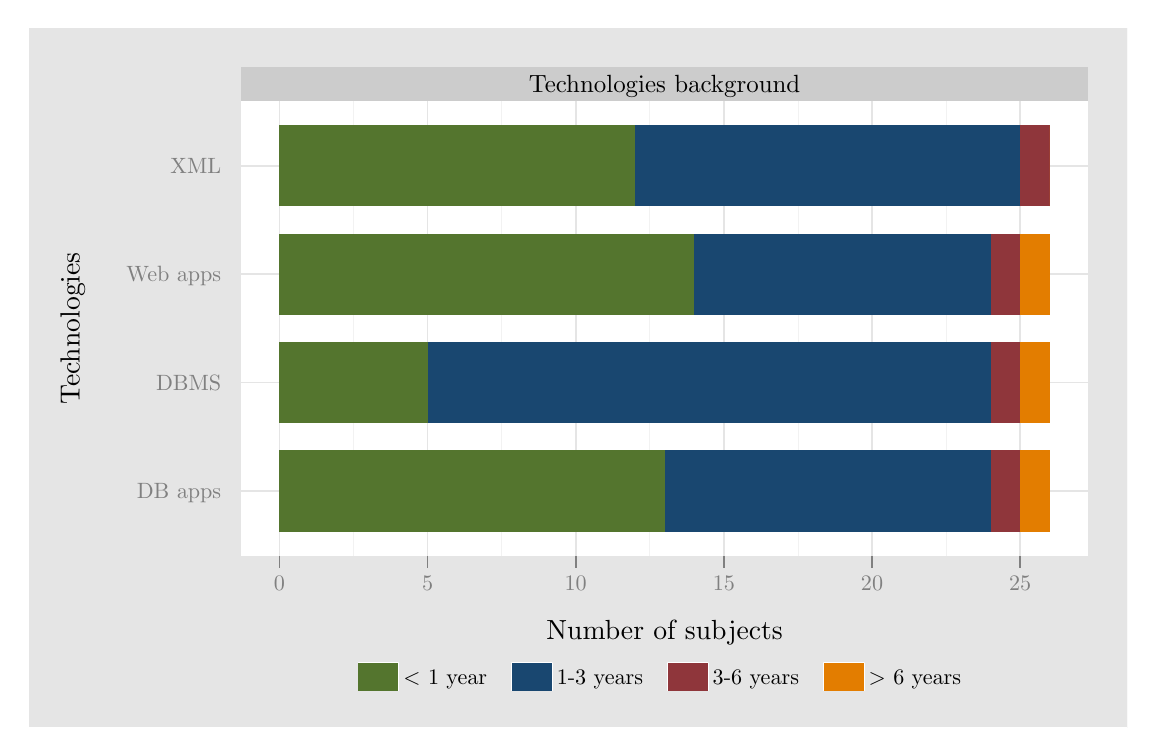
\begin{tikzpicture}[x=1pt,y=1pt]
\definecolor[named]{fillColor}{rgb}{1.00,1.00,1.00}
\path[use as bounding box,fill=fillColor,fill opacity=0.00] (0,0) rectangle (397.48,252.94);
\begin{scope}
\path[clip] (  0.00,  0.00) rectangle (397.48,252.94);
\definecolor[named]{drawColor}{rgb}{1.00,1.00,1.00}
\definecolor[named]{fillColor}{rgb}{0.90,0.90,0.90}

\path[draw=drawColor,line width= 0.6pt,line join=round,line cap=round,fill=fillColor] (  0.00,  0.00) rectangle (397.48,252.95);
\end{scope}
\begin{scope}
\path[clip] ( 77.04, 62.05) rectangle (383.26,226.50);
\definecolor[named]{fillColor}{rgb}{1.00,1.00,1.00}

\path[fill=fillColor] ( 77.04, 62.05) rectangle (383.26,226.50);
\definecolor[named]{drawColor}{rgb}{0.95,0.95,0.95}

\path[draw=drawColor,line width= 0.3pt,line join=round] (117.73, 62.05) --
	(117.73,226.50);

\path[draw=drawColor,line width= 0.3pt,line join=round] (171.26, 62.05) --
	(171.26,226.50);

\path[draw=drawColor,line width= 0.3pt,line join=round] (224.80, 62.05) --
	(224.80,226.50);

\path[draw=drawColor,line width= 0.3pt,line join=round] (278.33, 62.05) --
	(278.33,226.50);

\path[draw=drawColor,line width= 0.3pt,line join=round] (331.87, 62.05) --
	(331.87,226.50);
\definecolor[named]{drawColor}{rgb}{0.90,0.90,0.90}

\path[draw=drawColor,line width= 0.6pt,line join=round] ( 77.04, 85.54) --
	(383.26, 85.54);

\path[draw=drawColor,line width= 0.6pt,line join=round] ( 77.04,124.69) --
	(383.26,124.69);

\path[draw=drawColor,line width= 0.6pt,line join=round] ( 77.04,163.85) --
	(383.26,163.85);

\path[draw=drawColor,line width= 0.6pt,line join=round] ( 77.04,203.00) --
	(383.26,203.00);

\path[draw=drawColor,line width= 0.6pt,line join=round] ( 90.96, 62.05) --
	( 90.96,226.50);

\path[draw=drawColor,line width= 0.6pt,line join=round] (144.50, 62.05) --
	(144.50,226.50);

\path[draw=drawColor,line width= 0.6pt,line join=round] (198.03, 62.05) --
	(198.03,226.50);

\path[draw=drawColor,line width= 0.6pt,line join=round] (251.56, 62.05) --
	(251.56,226.50);

\path[draw=drawColor,line width= 0.6pt,line join=round] (305.10, 62.05) --
	(305.10,226.50);

\path[draw=drawColor,line width= 0.6pt,line join=round] (358.63, 62.05) --
	(358.63,226.50);
\definecolor[named]{fillColor}{rgb}{0.33,0.46,0.18}

\path[fill=fillColor] ( 90.96, 70.86) rectangle (230.15,100.22);
\definecolor[named]{fillColor}{rgb}{0.10,0.28,0.44}

\path[fill=fillColor] (230.15, 70.86) rectangle (347.93,100.22);
\definecolor[named]{fillColor}{rgb}{0.56,0.21,0.23}

\path[fill=fillColor] (347.93, 70.86) rectangle (358.63,100.22);
\definecolor[named]{fillColor}{rgb}{0.89,0.49,0.00}

\path[fill=fillColor] (358.63, 70.86) rectangle (369.34,100.22);
\definecolor[named]{fillColor}{rgb}{0.33,0.46,0.18}

\path[fill=fillColor] ( 90.96,110.01) rectangle (144.50,139.38);
\definecolor[named]{fillColor}{rgb}{0.10,0.28,0.44}

\path[fill=fillColor] (144.50,110.01) rectangle (347.93,139.38);
\definecolor[named]{fillColor}{rgb}{0.56,0.21,0.23}

\path[fill=fillColor] (347.93,110.01) rectangle (358.63,139.38);
\definecolor[named]{fillColor}{rgb}{0.89,0.49,0.00}

\path[fill=fillColor] (358.63,110.01) rectangle (369.34,139.38);
\definecolor[named]{fillColor}{rgb}{0.33,0.46,0.18}

\path[fill=fillColor] ( 90.96,149.17) rectangle (240.86,178.53);
\definecolor[named]{fillColor}{rgb}{0.10,0.28,0.44}

\path[fill=fillColor] (240.86,149.17) rectangle (347.93,178.53);
\definecolor[named]{fillColor}{rgb}{0.56,0.21,0.23}

\path[fill=fillColor] (347.93,149.17) rectangle (358.63,178.53);
\definecolor[named]{fillColor}{rgb}{0.89,0.49,0.00}

\path[fill=fillColor] (358.63,149.17) rectangle (369.34,178.53);
\definecolor[named]{fillColor}{rgb}{0.33,0.46,0.18}

\path[fill=fillColor] ( 90.96,188.32) rectangle (219.44,217.69);
\definecolor[named]{fillColor}{rgb}{0.10,0.28,0.44}

\path[fill=fillColor] (219.44,188.32) rectangle (358.63,217.69);
\definecolor[named]{fillColor}{rgb}{0.56,0.21,0.23}

\path[fill=fillColor] (358.63,188.32) rectangle (369.34,217.69);
\definecolor[named]{fillColor}{rgb}{0.89,0.49,0.00}

\path[fill=fillColor] (369.34,188.32) rectangle (369.34,217.69);
\end{scope}
\begin{scope}
\path[clip] (  0.00,  0.00) rectangle (397.48,252.94);
\definecolor[named]{fillColor}{rgb}{0.80,0.80,0.80}

\path[fill=fillColor] ( 77.04,226.50) rectangle (383.26,238.72);
\definecolor[named]{drawColor}{rgb}{0.00,0.00,0.00}

\node[text=drawColor,anchor=base,inner sep=0pt, outer sep=0pt, scale=  0.90] at (230.15,229.51) {Technologies background};
\end{scope}
\begin{scope}
\path[clip] (  0.00,  0.00) rectangle (397.48,252.94);
\definecolor[named]{drawColor}{rgb}{0.50,0.50,0.50}

\node[text=drawColor,anchor=base east,inner sep=0pt, outer sep=0pt, scale=  0.80] at ( 69.93, 82.79) {DB apps};

\node[text=drawColor,anchor=base east,inner sep=0pt, outer sep=0pt, scale=  0.80] at ( 69.93,121.94) {DBMS};

\node[text=drawColor,anchor=base east,inner sep=0pt, outer sep=0pt, scale=  0.80] at ( 69.93,161.09) {Web apps};

\node[text=drawColor,anchor=base east,inner sep=0pt, outer sep=0pt, scale=  0.80] at ( 69.93,200.25) {XML};
\end{scope}
\begin{scope}
\path[clip] (  0.00,  0.00) rectangle (397.48,252.94);
\definecolor[named]{drawColor}{rgb}{0.50,0.50,0.50}

\path[draw=drawColor,line width= 0.6pt,line join=round] ( 90.96, 57.78) --
	( 90.96, 62.05);

\path[draw=drawColor,line width= 0.6pt,line join=round] (144.50, 57.78) --
	(144.50, 62.05);

\path[draw=drawColor,line width= 0.6pt,line join=round] (198.03, 57.78) --
	(198.03, 62.05);

\path[draw=drawColor,line width= 0.6pt,line join=round] (251.56, 57.78) --
	(251.56, 62.05);

\path[draw=drawColor,line width= 0.6pt,line join=round] (305.10, 57.78) --
	(305.10, 62.05);

\path[draw=drawColor,line width= 0.6pt,line join=round] (358.63, 57.78) --
	(358.63, 62.05);
\end{scope}
\begin{scope}
\path[clip] (  0.00,  0.00) rectangle (397.48,252.94);
\definecolor[named]{drawColor}{rgb}{0.50,0.50,0.50}

\node[text=drawColor,anchor=base,inner sep=0pt, outer sep=0pt, scale=  0.80] at ( 90.96, 49.42) {0};

\node[text=drawColor,anchor=base,inner sep=0pt, outer sep=0pt, scale=  0.80] at (144.50, 49.42) {5};

\node[text=drawColor,anchor=base,inner sep=0pt, outer sep=0pt, scale=  0.80] at (198.03, 49.42) {10};

\node[text=drawColor,anchor=base,inner sep=0pt, outer sep=0pt, scale=  0.80] at (251.56, 49.42) {15};

\node[text=drawColor,anchor=base,inner sep=0pt, outer sep=0pt, scale=  0.80] at (305.10, 49.42) {20};

\node[text=drawColor,anchor=base,inner sep=0pt, outer sep=0pt, scale=  0.80] at (358.63, 49.42) {25};
\end{scope}
\begin{scope}
\path[clip] (  0.00,  0.00) rectangle (397.48,252.94);
\definecolor[named]{drawColor}{rgb}{0.00,0.00,0.00}

\node[text=drawColor,anchor=base,inner sep=0pt, outer sep=0pt, scale=  1.00] at (230.15, 31.70) {Number of subjects};
\end{scope}
\begin{scope}
\path[clip] (  0.00,  0.00) rectangle (397.48,252.94);
\definecolor[named]{drawColor}{rgb}{0.00,0.00,0.00}

\node[text=drawColor,rotate= 90.00,anchor=base,inner sep=0pt, outer sep=0pt, scale=  1.00] at ( 18.80,144.27) {Technologies};
\end{scope}
\begin{scope}
\path[clip] (  0.00,  0.00) rectangle (397.48,252.94);
\definecolor[named]{fillColor}{rgb}{0.90,0.90,0.90}

\path[fill=fillColor] (111.64,  9.15) rectangle (348.66, 27.65);
\end{scope}
\begin{scope}
\path[clip] (  0.00,  0.00) rectangle (397.48,252.94);
\definecolor[named]{drawColor}{rgb}{1.00,1.00,1.00}
\definecolor[named]{fillColor}{rgb}{1.00,1.00,1.00}

\path[draw=drawColor,line width= 0.6pt,line join=round,line cap=round,fill=fillColor] (119.52, 13.42) rectangle (133.97, 23.38);
\end{scope}
\begin{scope}
\path[clip] (  0.00,  0.00) rectangle (397.48,252.94);
\definecolor[named]{fillColor}{rgb}{0.33,0.46,0.18}

\path[fill=fillColor] (119.52, 13.42) rectangle (133.97, 23.38);

\path[] (119.52, 13.42) --
	(133.97, 23.38);
\end{scope}
\begin{scope}
\path[clip] (  0.00,  0.00) rectangle (397.48,252.94);
\definecolor[named]{drawColor}{rgb}{1.00,1.00,1.00}
\definecolor[named]{fillColor}{rgb}{1.00,1.00,1.00}

\path[draw=drawColor,line width= 0.6pt,line join=round,line cap=round,fill=fillColor] (174.94, 13.42) rectangle (189.39, 23.38);
\end{scope}
\begin{scope}
\path[clip] (  0.00,  0.00) rectangle (397.48,252.94);
\definecolor[named]{fillColor}{rgb}{0.10,0.28,0.44}

\path[fill=fillColor] (174.94, 13.42) rectangle (189.39, 23.38);

\path[] (174.94, 13.42) --
	(189.39, 23.38);
\end{scope}
\begin{scope}
\path[clip] (  0.00,  0.00) rectangle (397.48,252.94);
\definecolor[named]{drawColor}{rgb}{1.00,1.00,1.00}
\definecolor[named]{fillColor}{rgb}{1.00,1.00,1.00}

\path[draw=drawColor,line width= 0.6pt,line join=round,line cap=round,fill=fillColor] (231.28, 13.42) rectangle (245.74, 23.38);
\end{scope}
\begin{scope}
\path[clip] (  0.00,  0.00) rectangle (397.48,252.94);
\definecolor[named]{fillColor}{rgb}{0.56,0.21,0.23}

\path[fill=fillColor] (231.28, 13.42) rectangle (245.74, 23.38);

\path[] (231.28, 13.42) --
	(245.74, 23.38);
\end{scope}
\begin{scope}
\path[clip] (  0.00,  0.00) rectangle (397.48,252.94);
\definecolor[named]{drawColor}{rgb}{1.00,1.00,1.00}
\definecolor[named]{fillColor}{rgb}{1.00,1.00,1.00}

\path[draw=drawColor,line width= 0.6pt,line join=round,line cap=round,fill=fillColor] (287.63, 13.42) rectangle (302.09, 23.38);
\end{scope}
\begin{scope}
\path[clip] (  0.00,  0.00) rectangle (397.48,252.94);
\definecolor[named]{fillColor}{rgb}{0.89,0.49,0.00}

\path[fill=fillColor] (287.63, 13.42) rectangle (302.09, 23.38);

\path[] (287.63, 13.42) --
	(302.09, 23.38);
\end{scope}
\begin{scope}
\path[clip] (  0.00,  0.00) rectangle (397.48,252.94);
\definecolor[named]{drawColor}{rgb}{0.00,0.00,0.00}

\node[text=drawColor,anchor=base west,inner sep=0pt, outer sep=0pt, scale=  0.80] at (135.78, 15.64) {$<$ 1 year $\;\;$};
\end{scope}
\begin{scope}
\path[clip] (  0.00,  0.00) rectangle (397.48,252.94);
\definecolor[named]{drawColor}{rgb}{0.00,0.00,0.00}

\node[text=drawColor,anchor=base west,inner sep=0pt, outer sep=0pt, scale=  0.80] at (191.20, 15.64) {1-3 years $\;\;$};
\end{scope}
\begin{scope}
\path[clip] (  0.00,  0.00) rectangle (397.48,252.94);
\definecolor[named]{drawColor}{rgb}{0.00,0.00,0.00}

\node[text=drawColor,anchor=base west,inner sep=0pt, outer sep=0pt, scale=  0.80] at (247.54, 15.64) {3-6 years $\;\;$};
\end{scope}
\begin{scope}
\path[clip] (  0.00,  0.00) rectangle (397.48,252.94);
\definecolor[named]{drawColor}{rgb}{0.00,0.00,0.00}

\node[text=drawColor,anchor=base west,inner sep=0pt, outer sep=0pt, scale=  0.80] at (303.89, 15.64) {$>$ 6 years $\;\;$};
\end{scope}
\end{tikzpicture}

 }
 \caption[Survey participants' technological background]{Survey participants' background knowledge working with technologies relevant to the study.}
 \label{fig:experimentation:survey:background-technology-experience}
\end{figure}

\begin{figure}
 \centering
 \framebox[\textwidth]{
 % Created by tikzDevice version 0.6.2-92-0ad2792 on 2013-04-07 17:56:48
% !TEX encoding = UTF-8 Unicode
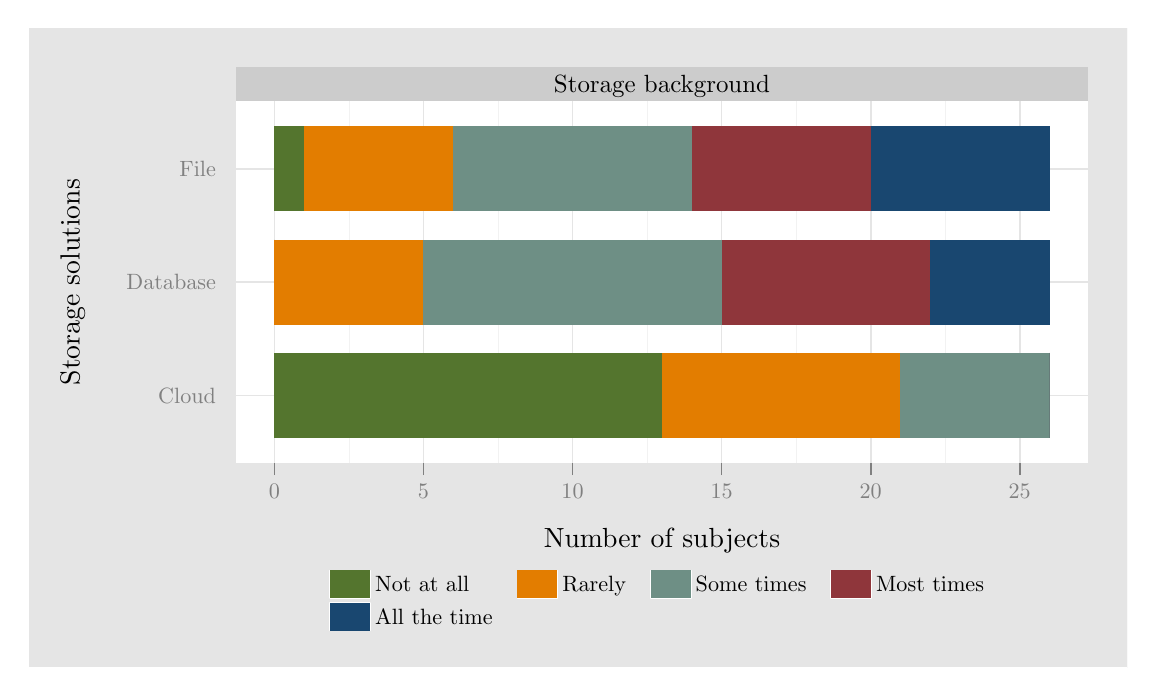
\begin{tikzpicture}[x=1pt,y=1pt]
\definecolor[named]{fillColor}{rgb}{1.00,1.00,1.00}
\path[use as bounding box,fill=fillColor,fill opacity=0.00] (0,0) rectangle (397.48,231.26);
\begin{scope}
\path[clip] (  0.00,  0.00) rectangle (397.48,231.26);
\definecolor[named]{drawColor}{rgb}{1.00,1.00,1.00}
\definecolor[named]{fillColor}{rgb}{0.90,0.90,0.90}

\path[draw=drawColor,line width= 0.6pt,line join=round,line cap=round,fill=fillColor] (  0.00,  0.00) rectangle (397.48,231.26);
\end{scope}
\begin{scope}
\path[clip] ( 75.16, 73.81) rectangle (383.26,204.82);
\definecolor[named]{fillColor}{rgb}{1.00,1.00,1.00}

\path[fill=fillColor] ( 75.16, 73.81) rectangle (383.26,204.82);
\definecolor[named]{drawColor}{rgb}{0.95,0.95,0.95}

\path[draw=drawColor,line width= 0.3pt,line join=round] (116.09, 73.81) --
	(116.09,204.82);

\path[draw=drawColor,line width= 0.3pt,line join=round] (169.96, 73.81) --
	(169.96,204.82);

\path[draw=drawColor,line width= 0.3pt,line join=round] (223.82, 73.81) --
	(223.82,204.82);

\path[draw=drawColor,line width= 0.3pt,line join=round] (277.68, 73.81) --
	(277.68,204.82);

\path[draw=drawColor,line width= 0.3pt,line join=round] (331.55, 73.81) --
	(331.55,204.82);
\definecolor[named]{drawColor}{rgb}{0.90,0.90,0.90}

\path[draw=drawColor,line width= 0.6pt,line join=round] ( 75.16, 98.38) --
	(383.26, 98.38);

\path[draw=drawColor,line width= 0.6pt,line join=round] ( 75.16,139.31) --
	(383.26,139.31);

\path[draw=drawColor,line width= 0.6pt,line join=round] ( 75.16,180.25) --
	(383.26,180.25);

\path[draw=drawColor,line width= 0.6pt,line join=round] ( 89.16, 73.81) --
	( 89.16,204.82);

\path[draw=drawColor,line width= 0.6pt,line join=round] (143.02, 73.81) --
	(143.02,204.82);

\path[draw=drawColor,line width= 0.6pt,line join=round] (196.89, 73.81) --
	(196.89,204.82);

\path[draw=drawColor,line width= 0.6pt,line join=round] (250.75, 73.81) --
	(250.75,204.82);

\path[draw=drawColor,line width= 0.6pt,line join=round] (304.62, 73.81) --
	(304.62,204.82);

\path[draw=drawColor,line width= 0.6pt,line join=round] (358.48, 73.81) --
	(358.48,204.82);
\definecolor[named]{fillColor}{rgb}{0.33,0.46,0.18}

\path[fill=fillColor] ( 89.16, 83.02) rectangle (229.21,113.73);
\definecolor[named]{fillColor}{rgb}{0.89,0.49,0.00}

\path[fill=fillColor] (229.21, 83.02) rectangle (315.39,113.73);
\definecolor[named]{fillColor}{rgb}{0.43,0.56,0.52}

\path[fill=fillColor] (315.39, 83.02) rectangle (369.25,113.73);
\definecolor[named]{fillColor}{rgb}{0.56,0.21,0.23}

\path[fill=fillColor] (369.25, 83.02) rectangle (369.25,113.73);
\definecolor[named]{fillColor}{rgb}{0.10,0.28,0.44}

\path[fill=fillColor] (369.25, 83.02) rectangle (369.25,113.73);
\definecolor[named]{fillColor}{rgb}{0.33,0.46,0.18}

\path[fill=fillColor] ( 89.16,123.96) rectangle ( 89.16,154.67);
\definecolor[named]{fillColor}{rgb}{0.89,0.49,0.00}

\path[fill=fillColor] ( 89.16,123.96) rectangle (143.02,154.67);
\definecolor[named]{fillColor}{rgb}{0.43,0.56,0.52}

\path[fill=fillColor] (143.02,123.96) rectangle (250.75,154.67);
\definecolor[named]{fillColor}{rgb}{0.56,0.21,0.23}

\path[fill=fillColor] (250.75,123.96) rectangle (326.16,154.67);
\definecolor[named]{fillColor}{rgb}{0.10,0.28,0.44}

\path[fill=fillColor] (326.16,123.96) rectangle (369.25,154.67);
\definecolor[named]{fillColor}{rgb}{0.33,0.46,0.18}

\path[fill=fillColor] ( 89.16,164.90) rectangle ( 99.93,195.61);
\definecolor[named]{fillColor}{rgb}{0.89,0.49,0.00}

\path[fill=fillColor] ( 99.93,164.90) rectangle (153.80,195.61);
\definecolor[named]{fillColor}{rgb}{0.43,0.56,0.52}

\path[fill=fillColor] (153.80,164.90) rectangle (239.98,195.61);
\definecolor[named]{fillColor}{rgb}{0.56,0.21,0.23}

\path[fill=fillColor] (239.98,164.90) rectangle (304.62,195.61);
\definecolor[named]{fillColor}{rgb}{0.10,0.28,0.44}

\path[fill=fillColor] (304.62,164.90) rectangle (369.25,195.61);
\end{scope}
\begin{scope}
\path[clip] (  0.00,  0.00) rectangle (397.48,231.26);
\definecolor[named]{fillColor}{rgb}{0.80,0.80,0.80}

\path[fill=fillColor] ( 75.16,204.82) rectangle (383.26,217.04);
\definecolor[named]{drawColor}{rgb}{0.00,0.00,0.00}

\node[text=drawColor,anchor=base,inner sep=0pt, outer sep=0pt, scale=  0.90] at (229.21,207.83) {Storage background};
\end{scope}
\begin{scope}
\path[clip] (  0.00,  0.00) rectangle (397.48,231.26);
\definecolor[named]{drawColor}{rgb}{0.50,0.50,0.50}

\node[text=drawColor,anchor=base east,inner sep=0pt, outer sep=0pt, scale=  0.80] at ( 68.04, 95.62) {Cloud};

\node[text=drawColor,anchor=base east,inner sep=0pt, outer sep=0pt, scale=  0.80] at ( 68.04,136.56) {Database};

\node[text=drawColor,anchor=base east,inner sep=0pt, outer sep=0pt, scale=  0.80] at ( 68.04,177.50) {File};
\end{scope}
\begin{scope}
\path[clip] (  0.00,  0.00) rectangle (397.48,231.26);
\definecolor[named]{drawColor}{rgb}{0.50,0.50,0.50}

\path[draw=drawColor,line width= 0.6pt,line join=round] ( 89.16, 69.54) --
	( 89.16, 73.81);

\path[draw=drawColor,line width= 0.6pt,line join=round] (143.02, 69.54) --
	(143.02, 73.81);

\path[draw=drawColor,line width= 0.6pt,line join=round] (196.89, 69.54) --
	(196.89, 73.81);

\path[draw=drawColor,line width= 0.6pt,line join=round] (250.75, 69.54) --
	(250.75, 73.81);

\path[draw=drawColor,line width= 0.6pt,line join=round] (304.62, 69.54) --
	(304.62, 73.81);

\path[draw=drawColor,line width= 0.6pt,line join=round] (358.48, 69.54) --
	(358.48, 73.81);
\end{scope}
\begin{scope}
\path[clip] (  0.00,  0.00) rectangle (397.48,231.26);
\definecolor[named]{drawColor}{rgb}{0.50,0.50,0.50}

\node[text=drawColor,anchor=base,inner sep=0pt, outer sep=0pt, scale=  0.80] at ( 89.16, 61.19) {0};

\node[text=drawColor,anchor=base,inner sep=0pt, outer sep=0pt, scale=  0.80] at (143.02, 61.19) {5};

\node[text=drawColor,anchor=base,inner sep=0pt, outer sep=0pt, scale=  0.80] at (196.89, 61.19) {10};

\node[text=drawColor,anchor=base,inner sep=0pt, outer sep=0pt, scale=  0.80] at (250.75, 61.19) {15};

\node[text=drawColor,anchor=base,inner sep=0pt, outer sep=0pt, scale=  0.80] at (304.62, 61.19) {20};

\node[text=drawColor,anchor=base,inner sep=0pt, outer sep=0pt, scale=  0.80] at (358.48, 61.19) {25};
\end{scope}
\begin{scope}
\path[clip] (  0.00,  0.00) rectangle (397.48,231.26);
\definecolor[named]{drawColor}{rgb}{0.00,0.00,0.00}

\node[text=drawColor,anchor=base,inner sep=0pt, outer sep=0pt, scale=  1.00] at (229.21, 43.46) {Number of subjects };
\end{scope}
\begin{scope}
\path[clip] (  0.00,  0.00) rectangle (397.48,231.26);
\definecolor[named]{drawColor}{rgb}{0.00,0.00,0.00}

\node[text=drawColor,rotate= 90.00,anchor=base,inner sep=0pt, outer sep=0pt, scale=  1.00] at ( 18.80,139.31) { Storage solutions};
\end{scope}
\begin{scope}
\path[clip] (  0.00,  0.00) rectangle (397.48,231.26);
\definecolor[named]{fillColor}{rgb}{0.90,0.90,0.90}

\path[fill=fillColor] (101.45,  9.15) rectangle (356.96, 39.41);
\end{scope}
\begin{scope}
\path[clip] (  0.00,  0.00) rectangle (397.48,231.26);
\definecolor[named]{drawColor}{rgb}{1.00,1.00,1.00}
\definecolor[named]{fillColor}{rgb}{1.00,1.00,1.00}

\path[draw=drawColor,line width= 0.6pt,line join=round,line cap=round,fill=fillColor] (109.33, 25.19) rectangle (123.79, 35.14);
\end{scope}
\begin{scope}
\path[clip] (  0.00,  0.00) rectangle (397.48,231.26);
\definecolor[named]{fillColor}{rgb}{0.33,0.46,0.18}

\path[fill=fillColor] (109.33, 25.19) rectangle (123.79, 35.14);

\path[] (109.33, 25.19) --
	(123.79, 35.14);
\end{scope}
\begin{scope}
\path[clip] (  0.00,  0.00) rectangle (397.48,231.26);
\definecolor[named]{drawColor}{rgb}{1.00,1.00,1.00}
\definecolor[named]{fillColor}{rgb}{1.00,1.00,1.00}

\path[draw=drawColor,line width= 0.6pt,line join=round,line cap=round,fill=fillColor] (176.95, 25.19) rectangle (191.40, 35.14);
\end{scope}
\begin{scope}
\path[clip] (  0.00,  0.00) rectangle (397.48,231.26);
\definecolor[named]{fillColor}{rgb}{0.89,0.49,0.00}

\path[fill=fillColor] (176.95, 25.19) rectangle (191.40, 35.14);

\path[] (176.95, 25.19) --
	(191.40, 35.14);
\end{scope}
\begin{scope}
\path[clip] (  0.00,  0.00) rectangle (397.48,231.26);
\definecolor[named]{drawColor}{rgb}{1.00,1.00,1.00}
\definecolor[named]{fillColor}{rgb}{1.00,1.00,1.00}

\path[draw=drawColor,line width= 0.6pt,line join=round,line cap=round,fill=fillColor] (225.14, 25.19) rectangle (239.59, 35.14);
\end{scope}
\begin{scope}
\path[clip] (  0.00,  0.00) rectangle (397.48,231.26);
\definecolor[named]{fillColor}{rgb}{0.43,0.56,0.52}

\path[fill=fillColor] (225.14, 25.19) rectangle (239.59, 35.14);

\path[] (225.14, 25.19) --
	(239.59, 35.14);
\end{scope}
\begin{scope}
\path[clip] (  0.00,  0.00) rectangle (397.48,231.26);
\definecolor[named]{drawColor}{rgb}{1.00,1.00,1.00}
\definecolor[named]{fillColor}{rgb}{1.00,1.00,1.00}

\path[draw=drawColor,line width= 0.6pt,line join=round,line cap=round,fill=fillColor] (290.35, 25.19) rectangle (304.81, 35.14);
\end{scope}
\begin{scope}
\path[clip] (  0.00,  0.00) rectangle (397.48,231.26);
\definecolor[named]{fillColor}{rgb}{0.56,0.21,0.23}

\path[fill=fillColor] (290.35, 25.19) rectangle (304.81, 35.14);

\path[] (290.35, 25.19) --
	(304.81, 35.14);
\end{scope}
\begin{scope}
\path[clip] (  0.00,  0.00) rectangle (397.48,231.26);
\definecolor[named]{drawColor}{rgb}{1.00,1.00,1.00}
\definecolor[named]{fillColor}{rgb}{1.00,1.00,1.00}

\path[draw=drawColor,line width= 0.6pt,line join=round,line cap=round,fill=fillColor] (109.33, 13.42) rectangle (123.79, 23.38);
\end{scope}
\begin{scope}
\path[clip] (  0.00,  0.00) rectangle (397.48,231.26);
\definecolor[named]{fillColor}{rgb}{0.10,0.28,0.44}

\path[fill=fillColor] (109.33, 13.42) rectangle (123.79, 23.38);

\path[] (109.33, 13.42) --
	(123.79, 23.38);
\end{scope}
\begin{scope}
\path[clip] (  0.00,  0.00) rectangle (397.48,231.26);
\definecolor[named]{drawColor}{rgb}{0.00,0.00,0.00}

\node[text=drawColor,anchor=base west,inner sep=0pt, outer sep=0pt, scale=  0.80] at (125.59, 27.41) {Not at all $\;\;$};
\end{scope}
\begin{scope}
\path[clip] (  0.00,  0.00) rectangle (397.48,231.26);
\definecolor[named]{drawColor}{rgb}{0.00,0.00,0.00}

\node[text=drawColor,anchor=base west,inner sep=0pt, outer sep=0pt, scale=  0.80] at (193.21, 27.41) {Rarely $\;\;$};
\end{scope}
\begin{scope}
\path[clip] (  0.00,  0.00) rectangle (397.48,231.26);
\definecolor[named]{drawColor}{rgb}{0.00,0.00,0.00}

\node[text=drawColor,anchor=base west,inner sep=0pt, outer sep=0pt, scale=  0.80] at (241.40, 27.41) {Some times $\;\;$};
\end{scope}
\begin{scope}
\path[clip] (  0.00,  0.00) rectangle (397.48,231.26);
\definecolor[named]{drawColor}{rgb}{0.00,0.00,0.00}

\node[text=drawColor,anchor=base west,inner sep=0pt, outer sep=0pt, scale=  0.80] at (306.61, 27.41) {Most times $\;\;$};
\end{scope}
\begin{scope}
\path[clip] (  0.00,  0.00) rectangle (397.48,231.26);
\definecolor[named]{drawColor}{rgb}{0.00,0.00,0.00}

\node[text=drawColor,anchor=base west,inner sep=0pt, outer sep=0pt, scale=  0.80] at (125.59, 15.64) {All the time $\;\;$};
\end{scope}
\end{tikzpicture}

 }
 \caption[Survey participants' background using storage solutions]{Survey participants' background working with some selected popular storage solutions.}
 \label{fig:experimentation:survey:background-storage-usage-frequency}
\end{figure}

\begin{figure}
 \centering
 \framebox[\textwidth]{
 % Created by tikzDevice version 0.6.2-92-0ad2792 on 2013-04-07 17:57:35
% !TEX encoding = UTF-8 Unicode
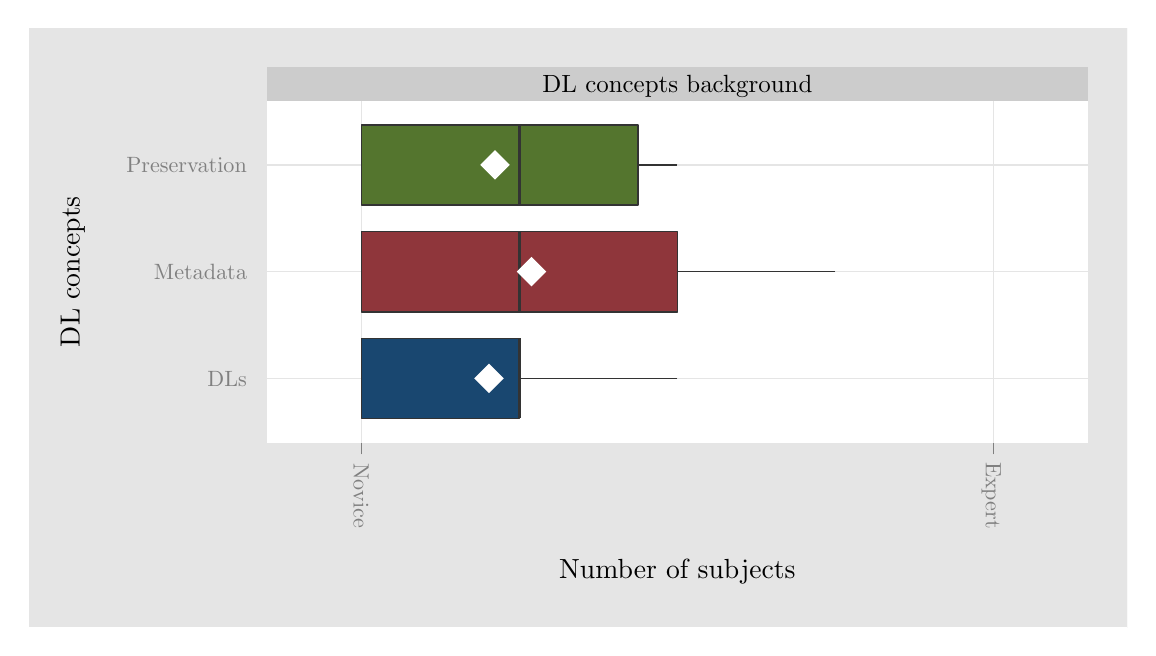
\begin{tikzpicture}[x=1pt,y=1pt]
\definecolor[named]{fillColor}{rgb}{1.00,1.00,1.00}
\path[use as bounding box,fill=fillColor,fill opacity=0.00] (0,0) rectangle (397.48,216.81);
\begin{scope}
\path[clip] (  0.00,  0.00) rectangle (397.48,216.81);
\definecolor[named]{drawColor}{rgb}{1.00,1.00,1.00}
\definecolor[named]{fillColor}{rgb}{0.90,0.90,0.90}

\path[draw=drawColor,line width= 0.6pt,line join=round,line cap=round,fill=fillColor] (  0.00,  0.00) rectangle (397.48,216.81);
\end{scope}
\begin{scope}
\path[clip] ( 86.31, 66.91) rectangle (383.26,190.36);
\definecolor[named]{fillColor}{rgb}{1.00,1.00,1.00}

\path[fill=fillColor] ( 86.31, 66.91) rectangle (383.26,190.36);
\definecolor[named]{drawColor}{rgb}{0.90,0.90,0.90}

\path[draw=drawColor,line width= 0.6pt,line join=round] ( 86.31, 90.06) --
	(383.26, 90.06);

\path[draw=drawColor,line width= 0.6pt,line join=round] ( 86.31,128.64) --
	(383.26,128.64);

\path[draw=drawColor,line width= 0.6pt,line join=round] ( 86.31,167.22) --
	(383.26,167.22);

\path[draw=drawColor,line width= 0.6pt,line join=round] (120.57, 66.91) --
	(120.57,190.36);

\path[draw=drawColor,line width= 0.6pt,line join=round] (349.00, 66.91) --
	(349.00,190.36);
\definecolor[named]{drawColor}{rgb}{0.20,0.20,0.20}
\definecolor[named]{fillColor}{rgb}{0.20,0.20,0.20}

\path[draw=drawColor,line width= 0.6pt,line join=round,fill=fillColor] (177.68, 90.06) -- (234.78, 90.06);

\path[draw=drawColor,line width= 0.6pt,line join=round,fill=fillColor] (120.57, 90.06) -- (120.57, 90.06);
\definecolor[named]{fillColor}{rgb}{0.10,0.28,0.44}

\path[draw=drawColor,line width= 0.6pt,line join=round,line cap=round,fill=fillColor] (177.68, 75.59) --
	(120.57, 75.59) --
	(120.57,104.53) --
	(177.68,104.53) --
	(177.68, 75.59) --
	cycle;
\definecolor[named]{fillColor}{rgb}{0.20,0.20,0.20}

\path[draw=drawColor,line width= 1.1pt,line join=round,fill=fillColor] (177.68, 75.59) -- (177.68,104.53);

\path[draw=drawColor,line width= 0.6pt,line join=round,fill=fillColor] (234.78,128.64) -- (291.89,128.64);

\path[draw=drawColor,line width= 0.6pt,line join=round,fill=fillColor] (120.57,128.64) -- (120.57,128.64);
\definecolor[named]{fillColor}{rgb}{0.56,0.21,0.23}

\path[draw=drawColor,line width= 0.6pt,line join=round,line cap=round,fill=fillColor] (234.78,114.17) --
	(120.57,114.17) --
	(120.57,143.10) --
	(234.78,143.10) --
	(234.78,114.17) --
	cycle;
\definecolor[named]{fillColor}{rgb}{0.20,0.20,0.20}

\path[draw=drawColor,line width= 1.1pt,line join=round,fill=fillColor] (177.68,114.17) -- (177.68,143.10);

\path[draw=drawColor,line width= 0.6pt,line join=round,fill=fillColor] (220.51,167.22) -- (234.78,167.22);

\path[draw=drawColor,line width= 0.6pt,line join=round,fill=fillColor] (120.57,167.22) -- (120.57,167.22);
\definecolor[named]{fillColor}{rgb}{0.33,0.46,0.18}

\path[draw=drawColor,line width= 0.6pt,line join=round,line cap=round,fill=fillColor] (220.51,152.75) --
	(120.57,152.75) --
	(120.57,181.68) --
	(220.51,181.68) --
	(220.51,152.75) --
	cycle;
\definecolor[named]{fillColor}{rgb}{0.20,0.20,0.20}

\path[draw=drawColor,line width= 1.1pt,line join=round,fill=fillColor] (177.68,152.75) -- (177.68,181.68);
\definecolor[named]{fillColor}{rgb}{1.00,1.00,1.00}

\path[fill=fillColor] (161.36, 90.06) --
	(166.70, 95.39) --
	(172.03, 90.06) --
	(166.70, 84.72) --
	cycle;

\path[fill=fillColor] (176.74,128.64) --
	(182.07,133.97) --
	(187.41,128.64) --
	(182.07,123.30) --
	cycle;

\path[fill=fillColor] (163.56,167.22) --
	(168.89,172.55) --
	(174.23,167.22) --
	(168.89,161.88) --
	cycle;
\end{scope}
\begin{scope}
\path[clip] (  0.00,  0.00) rectangle (397.48,216.81);
\definecolor[named]{fillColor}{rgb}{0.80,0.80,0.80}

\path[fill=fillColor] ( 86.31,190.36) rectangle (383.26,202.58);
\definecolor[named]{drawColor}{rgb}{0.00,0.00,0.00}

\node[text=drawColor,anchor=base,inner sep=0pt, outer sep=0pt, scale=  0.90] at (234.78,193.37) {DL concepts background};
\end{scope}
\begin{scope}
\path[clip] (  0.00,  0.00) rectangle (397.48,216.81);
\definecolor[named]{drawColor}{rgb}{0.50,0.50,0.50}

\node[text=drawColor,anchor=base east,inner sep=0pt, outer sep=0pt, scale=  0.80] at ( 79.19, 87.30) {DLs};

\node[text=drawColor,anchor=base east,inner sep=0pt, outer sep=0pt, scale=  0.80] at ( 79.19,125.88) {Metadata};

\node[text=drawColor,anchor=base east,inner sep=0pt, outer sep=0pt, scale=  0.80] at ( 79.19,164.46) {Preservation};
\end{scope}
\begin{scope}
\path[clip] (  0.00,  0.00) rectangle (397.48,216.81);
\definecolor[named]{drawColor}{rgb}{0.50,0.50,0.50}

\path[draw=drawColor,line width= 0.6pt,line join=round] (120.57, 62.64) --
	(120.57, 66.91);

\path[draw=drawColor,line width= 0.6pt,line join=round] (349.00, 62.64) --
	(349.00, 66.91);
\end{scope}
\begin{scope}
\path[clip] (  0.00,  0.00) rectangle (397.48,216.81);
\definecolor[named]{drawColor}{rgb}{0.50,0.50,0.50}

\node[text=drawColor,rotate=270.00,anchor=base,inner sep=0pt, outer sep=0pt, scale=  0.80] at (117.82, 47.74) {Novice};

\node[text=drawColor,rotate=270.00,anchor=base,inner sep=0pt, outer sep=0pt, scale=  0.80] at (346.24, 47.74) {Expert};
\end{scope}
\begin{scope}
\path[clip] (  0.00,  0.00) rectangle (397.48,216.81);
\definecolor[named]{drawColor}{rgb}{0.00,0.00,0.00}

\node[text=drawColor,anchor=base,inner sep=0pt, outer sep=0pt, scale=  1.00] at (234.78, 17.94) {Number of subjects};
\end{scope}
\begin{scope}
\path[clip] (  0.00,  0.00) rectangle (397.48,216.81);
\definecolor[named]{drawColor}{rgb}{0.00,0.00,0.00}

\node[text=drawColor,rotate= 90.00,anchor=base,inner sep=0pt, outer sep=0pt, scale=  1.00] at ( 18.80,128.64) {DL concepts};
\end{scope}
\end{tikzpicture}

 }
 \caption[Survey participants' knowledge of DL concepts]{Survey participants' knowledge of some fundamental DL concepts.}
 \label{fig:experimentation:survey:background-dl-concepts-skill-level}
\end{figure}

\begin{figure}
 \centering
 \framebox[\textwidth]{
 % Created by tikzDevice version 0.6.2-92-0ad2792 on 2013-04-07 17:58:07
% !TEX encoding = UTF-8 Unicode
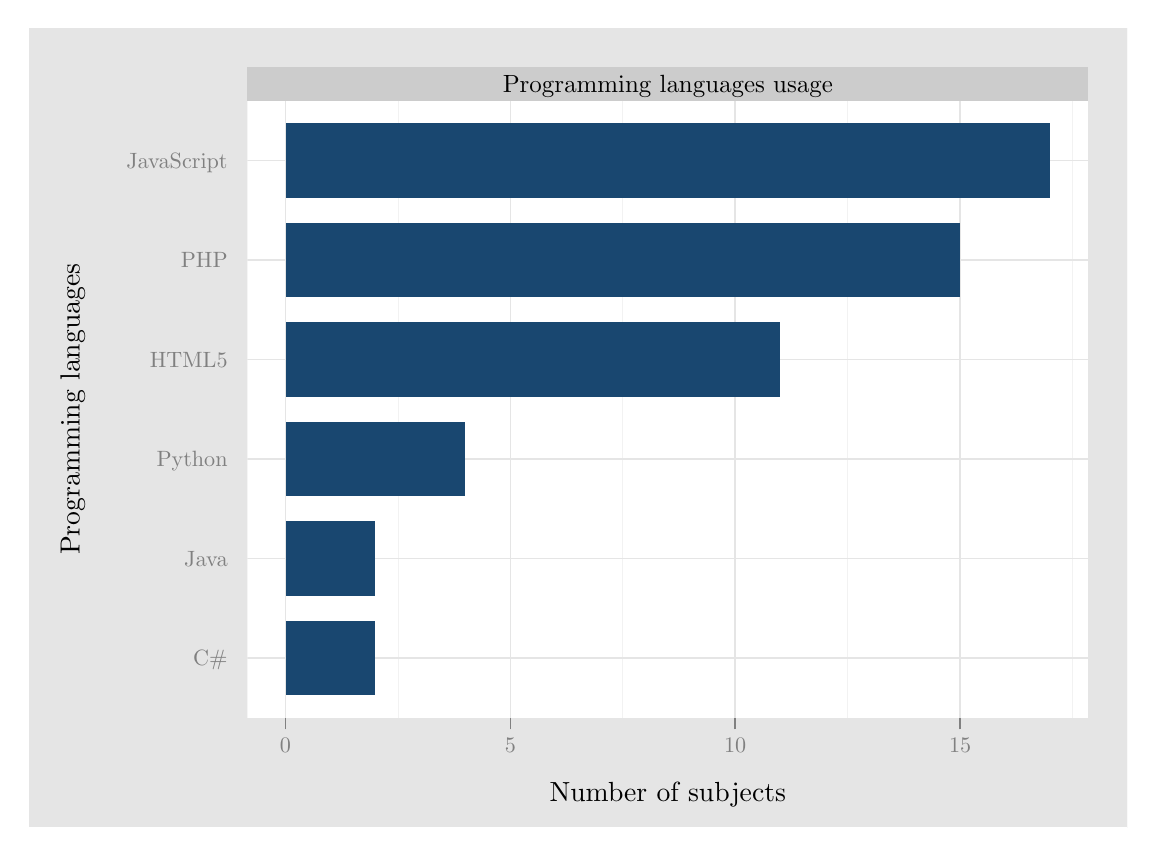
\begin{tikzpicture}[x=1pt,y=1pt]
\definecolor[named]{fillColor}{rgb}{1.00,1.00,1.00}
\path[use as bounding box,fill=fillColor,fill opacity=0.00] (0,0) rectangle (397.48,289.08);
\begin{scope}
\path[clip] (  0.00,  0.00) rectangle (397.48,289.08);
\definecolor[named]{drawColor}{rgb}{1.00,1.00,1.00}
\definecolor[named]{fillColor}{rgb}{0.90,0.90,0.90}

\path[draw=drawColor,line width= 0.6pt,line join=round,line cap=round,fill=fillColor] (  0.00, -0.00) rectangle (397.48,289.08);
\end{scope}
\begin{scope}
\path[clip] ( 79.35, 39.76) rectangle (383.26,262.63);
\definecolor[named]{fillColor}{rgb}{1.00,1.00,1.00}

\path[fill=fillColor] ( 79.35, 39.76) rectangle (383.26,262.63);
\definecolor[named]{drawColor}{rgb}{0.95,0.95,0.95}

\path[draw=drawColor,line width= 0.3pt,line join=round] (133.80, 39.76) --
	(133.80,262.63);

\path[draw=drawColor,line width= 0.3pt,line join=round] (215.05, 39.76) --
	(215.05,262.63);

\path[draw=drawColor,line width= 0.3pt,line join=round] (296.31, 39.76) --
	(296.31,262.63);

\path[draw=drawColor,line width= 0.3pt,line join=round] (377.57, 39.76) --
	(377.57,262.63);
\definecolor[named]{drawColor}{rgb}{0.90,0.90,0.90}

\path[draw=drawColor,line width= 0.6pt,line join=round] ( 79.35, 61.33) --
	(383.26, 61.33);

\path[draw=drawColor,line width= 0.6pt,line join=round] ( 79.35, 97.27) --
	(383.26, 97.27);

\path[draw=drawColor,line width= 0.6pt,line join=round] ( 79.35,133.22) --
	(383.26,133.22);

\path[draw=drawColor,line width= 0.6pt,line join=round] ( 79.35,169.17) --
	(383.26,169.17);

\path[draw=drawColor,line width= 0.6pt,line join=round] ( 79.35,205.12) --
	(383.26,205.12);

\path[draw=drawColor,line width= 0.6pt,line join=round] ( 79.35,241.06) --
	(383.26,241.06);

\path[draw=drawColor,line width= 0.6pt,line join=round] ( 93.17, 39.76) --
	( 93.17,262.63);

\path[draw=drawColor,line width= 0.6pt,line join=round] (174.43, 39.76) --
	(174.43,262.63);

\path[draw=drawColor,line width= 0.6pt,line join=round] (255.68, 39.76) --
	(255.68,262.63);

\path[draw=drawColor,line width= 0.6pt,line join=round] (336.94, 39.76) --
	(336.94,262.63);
\definecolor[named]{fillColor}{rgb}{0.10,0.28,0.44}

\path[fill=fillColor] ( 93.17, 47.85) rectangle (125.67, 74.81);

\path[fill=fillColor] ( 93.17, 83.79) rectangle (125.67,110.76);

\path[fill=fillColor] ( 93.17,119.74) rectangle (158.17,146.70);

\path[fill=fillColor] ( 93.17,155.69) rectangle (271.94,182.65);

\path[fill=fillColor] ( 93.17,191.64) rectangle (336.94,218.60);

\path[fill=fillColor] ( 93.17,227.58) rectangle (369.44,254.54);
\end{scope}
\begin{scope}
\path[clip] (  0.00,  0.00) rectangle (397.48,289.08);
\definecolor[named]{fillColor}{rgb}{0.80,0.80,0.80}

\path[fill=fillColor] ( 79.35,262.63) rectangle (383.26,274.85);
\definecolor[named]{drawColor}{rgb}{0.00,0.00,0.00}

\node[text=drawColor,anchor=base,inner sep=0pt, outer sep=0pt, scale=  0.90] at (231.31,265.64) {Programming languages usage};
\end{scope}
\begin{scope}
\path[clip] (  0.00,  0.00) rectangle (397.48,289.08);
\definecolor[named]{drawColor}{rgb}{0.50,0.50,0.50}

\node[text=drawColor,anchor=base east,inner sep=0pt, outer sep=0pt, scale=  0.80] at ( 72.24, 58.57) {C\#};

\node[text=drawColor,anchor=base east,inner sep=0pt, outer sep=0pt, scale=  0.80] at ( 72.24, 94.52) {Java};

\node[text=drawColor,anchor=base east,inner sep=0pt, outer sep=0pt, scale=  0.80] at ( 72.24,130.47) {Python};

\node[text=drawColor,anchor=base east,inner sep=0pt, outer sep=0pt, scale=  0.80] at ( 72.24,166.41) {HTML5};

\node[text=drawColor,anchor=base east,inner sep=0pt, outer sep=0pt, scale=  0.80] at ( 72.24,202.36) {PHP};

\node[text=drawColor,anchor=base east,inner sep=0pt, outer sep=0pt, scale=  0.80] at ( 72.24,238.31) {JavaScript};
\end{scope}
\begin{scope}
\path[clip] (  0.00,  0.00) rectangle (397.48,289.08);
\definecolor[named]{drawColor}{rgb}{0.50,0.50,0.50}

\path[draw=drawColor,line width= 0.6pt,line join=round] ( 93.17, 35.49) --
	( 93.17, 39.76);

\path[draw=drawColor,line width= 0.6pt,line join=round] (174.43, 35.49) --
	(174.43, 39.76);

\path[draw=drawColor,line width= 0.6pt,line join=round] (255.68, 35.49) --
	(255.68, 39.76);

\path[draw=drawColor,line width= 0.6pt,line join=round] (336.94, 35.49) --
	(336.94, 39.76);
\end{scope}
\begin{scope}
\path[clip] (  0.00,  0.00) rectangle (397.48,289.08);
\definecolor[named]{drawColor}{rgb}{0.50,0.50,0.50}

\node[text=drawColor,anchor=base,inner sep=0pt, outer sep=0pt, scale=  0.80] at ( 93.17, 27.14) {0};

\node[text=drawColor,anchor=base,inner sep=0pt, outer sep=0pt, scale=  0.80] at (174.43, 27.14) {5};

\node[text=drawColor,anchor=base,inner sep=0pt, outer sep=0pt, scale=  0.80] at (255.68, 27.14) {10};

\node[text=drawColor,anchor=base,inner sep=0pt, outer sep=0pt, scale=  0.80] at (336.94, 27.14) {15};
\end{scope}
\begin{scope}
\path[clip] (  0.00,  0.00) rectangle (397.48,289.08);
\definecolor[named]{drawColor}{rgb}{0.00,0.00,0.00}

\node[text=drawColor,anchor=base,inner sep=0pt, outer sep=0pt, scale=  1.00] at (231.31,  9.41) {Number of subjects};
\end{scope}
\begin{scope}
\path[clip] (  0.00,  0.00) rectangle (397.48,289.08);
\definecolor[named]{drawColor}{rgb}{0.00,0.00,0.00}

\node[text=drawColor,rotate= 90.00,anchor=base,inner sep=0pt, outer sep=0pt, scale=  1.00] at ( 18.80,151.20) {Programming languages};
\end{scope}
\end{tikzpicture}

 }
 \caption[Survey participants' programming languages usage]{Survey participants programming languages usage during service implementation.}
 \label{fig:experimentation:survey:programming-language-usage}
\end{figure}

\subsection{Results}
\label{sec:evaluation:developer-survey:results}

The survey participants' background-related information is shown in Figures~\ref{fig:experimentation:survey:background-technology-experience},~\ref{fig:experimentation:survey:background-storage-usage-frequency} and~\ref{fig:experimentation:survey:background-dl-concepts-skill-level}. The implementation of the Web services was done using a variety of programming languages, as shown in Figure~\ref{fig:experimentation:survey:programming-language-usage}.

The respondents' views on the simplicity\index{Simplicity} and ease of use of the repository\index{Repository} is shown in~\ref{fig:experimentation:survey:simplicity-understandability}; additionally, their rankings of possible storage solutions for metadata\index{Metadata} records are shown in Figure~\ref{fig:experimentation:survey:storage-solutions-ranking}. Finally, their preferences on the possible solutions to use for data management tasks/operations are shown in Figure~\ref{fig:experimentation:survey:data-management-operations}.

%%\subsubsection{Programming Language Support}
%%\label{sec:evaluation:developer-survey:results:extensibility}
%
% commented out due to duplication with plot...
%\tablespacing
%%%%%%\begin{longtable}{p{0.10\linewidth} p{0.040\linewidth}
%%%%%p{0.040\linewidth} p{0.040\linewidth} p{0.040\linewidth} p{0.040\linewidth}
%%%%%p{0.040\linewidth} p{0.040\linewidth} p{0.040\linewidth} p{0.040\linewidth}
%%%%%p{0.040\linewidth} p{0.040\linewidth} p {0.040\linewidth}}

\begin{longtable}{
>{\arraybackslash}p{0.18\linewidth}|
>{\centering\arraybackslash}p{0.035\linewidth}|
>{\centering\arraybackslash}p{0.035\linewidth}|
>{\centering\arraybackslash}p{0.035\linewidth}|
>{\centering\arraybackslash}p{0.035\linewidth}|
>{\centering\arraybackslash}p{0.035\linewidth}|
>{\centering\arraybackslash}p{0.035\linewidth}|
>{\centering\arraybackslash}p{0.035\linewidth}|
>{\centering\arraybackslash}p{0.035\linewidth}|
>{\centering\arraybackslash}p{0.035\linewidth}|
>{\centering\arraybackslash}p{0.035\linewidth}|
>{\centering\arraybackslash}p{0.035\linewidth}|
>{\centering\arraybackslash}p{0.035\linewidth}}

 \caption{Programming languages prevalence in practical assignment }
\label{tab:experimentation:survey:programming-language-usage}\\
 %%%%%\toprule
 %%%%%\cline{2-13}
 %%{} & \multicolumn{11}{c}{\textbf{Practical Assignment Group}}\\
 %%\midrule
 %%\textbf{Language} & 
 %%%%%\multicolumn{1}{c|}{} &
 \textbf{} &
 \multicolumn{1}{c|}{\begin{sideways}\textbf{Group 1}\end{sideways}} &
 \multicolumn{1}{c|}{\begin{sideways}\textbf{Group 2}\end{sideways}} &
 \multicolumn{1}{c|}{\begin{sideways}\textbf{Group 3}\end{sideways}} &
 \multicolumn{1}{c|}{\begin{sideways}\textbf{Group 4}\end{sideways}} &
 \multicolumn{1}{c|}{\begin{sideways}\textbf{Group 5}\end{sideways}} &
 \multicolumn{1}{c|}{\begin{sideways}\textbf{Group 6}\end{sideways}} &
 \multicolumn{1}{c|}{\begin{sideways}\textbf{Group 7}\end{sideways}} &
 \multicolumn{1}{c|}{\begin{sideways}\textbf{Group 8}\end{sideways}} &
 \multicolumn{1}{c|}{\begin{sideways}\textbf{Group 9}\end{sideways}} &
 \multicolumn{1}{c|}{\begin{sideways}\textbf{Group 10}\end{sideways}} &
 \multicolumn{1}{c|}{\begin{sideways}\textbf{Group 11}\end{sideways}} &
 \multicolumn{1}{c}{\begin{sideways}\textbf{Group 12}\end{sideways}}\\
 %%%%%\midrule
 \cline{1-13}
 \endfirsthead
 
 \caption[]{(continued)}\\
 %%%%%\toprule
 %%%%%\cline{2-13}
 %%{} & \multicolumn{12}{c}{\textbf{Programming Group}}\\
 %%\midrule
 %%\textbf{Language} & 
 %%%%%\multicolumn{1}{c|}{} &
 \textbf{} &
 \multicolumn{1}{c}{\begin{sideways}\textbf{Group 1}\end{sideways}} &
 \multicolumn{1}{c}{\begin{sideways}\textbf{Group 2}\end{sideways}} &
 \multicolumn{1}{c}{\begin{sideways}\textbf{Group 3}\end{sideways}} &
 \multicolumn{1}{c}{\begin{sideways}\textbf{Group 4}\end{sideways}} &
 \multicolumn{1}{c}{\begin{sideways}\textbf{Group 5}\end{sideways}} &
 \multicolumn{1}{c}{\begin{sideways}\textbf{Group 6}\end{sideways}} &
 \multicolumn{1}{c}{\begin{sideways}\textbf{Group 7}\end{sideways}} &
 \multicolumn{1}{c}{\begin{sideways}\textbf{Group 8}\end{sideways}} &
 \multicolumn{1}{c}{\begin{sideways}\textbf{Group 9}\end{sideways}} &
 \multicolumn{1}{c}{\begin{sideways}\textbf{Group 10}\end{sideways}} &
 \multicolumn{1}{c}{\begin{sideways}\textbf{Group 11}\end{sideways}} &
 \multicolumn{1}{c}{\begin{sideways}\textbf{Group 12}\end{sideways}}\\
 %%%%%\midrule
 \cline{1-13}
 \endhead
 
 % Page footer
 %%%%%\midrule
 \cline{1-13}
 \multicolumn{9}{r}{(Continued on next page)} \\
 \endfoot
 
 % Last page footer
 %%%%%\bottomrule
 \endlastfoot
 
 %   &
 \textbf{C\#}\index{C\#}&
 {}&
 {}&
 {}&
 {}&
 {}&
 {}&
 {}&
 {}&
 {}&
 {}&
 {X}&
 {}\\
 
 \cline{2-13}
 %\cmidrule[0.1pt](l{0.5em}r{0.5em}){1-13}
 
 %  &
 \textbf{HTML 5}\index{HTML 5}&
 {}&
 {}&
 {}&
 {}&
 {}&
 {X}&
 {X}&
 {X}&
 {X}&
 {}&
 {}&
 {X}\\
 
 \cline{2-13}
 %\cmidrule[0.1pt](l{0.5em}r{0.5em}){1-13}
 
 %&
 \textbf{Java}\index{Java}&
 {}&
 {}&
 {}&
 {}&
 {}&
 {X}&
 {}&
 {}&
 {}&
 {}&
 {}&
 {}\\
 
 \cline{2-13}
 %\cmidrule[0.1pt](l{0.5em}r{0.5em}){1-13}
  
 %&
 \textbf{JavaScript}\index{JavaScript}&
 {}&
 {X}&
 {X}&
 {X}&
 {}&
 {X}&
 {X}&
 {X}&
 {X}&
 {X}&
 {}&
 {}\\
 
 \cline{2-13}
 %\cmidrule[0.1pt](l{0.5em}r{0.5em}){1-13}
 
 %\begin{sideways}\textbf{Storage} \end{sideways} &
 %\begin{sideways}\textbf{} \end{sideways} &
 \textbf{PHP}\index{PHP}&
 {}&
 {X}&
 {X}&
 {}&
 {}&
 {X}&
 {}&
 {X}&
 {X}&
 {X}&
 {}&
 {X}\\
 
 \cline{2-13}
 %\cmidrule[0.1pt](l{0.5em}r{0.5em}){1-13}
 
 % &
 \textbf{Python}\index{Python}&
 {X}&
 {}&
 {}&
 {}&
 {X}&
 {}&
 {}&
 {}&
 {}&
 {}&
 {}&
 {}\\
 
\end{longtable}

%\bodyspacing

\begin{figure}
 \centering
 \framebox[\textwidth]{
 % Created by tikzDevice version 0.6.2-92-0ad2792 on 2013-04-07 23:42:51
% !TEX encoding = UTF-8 Unicode
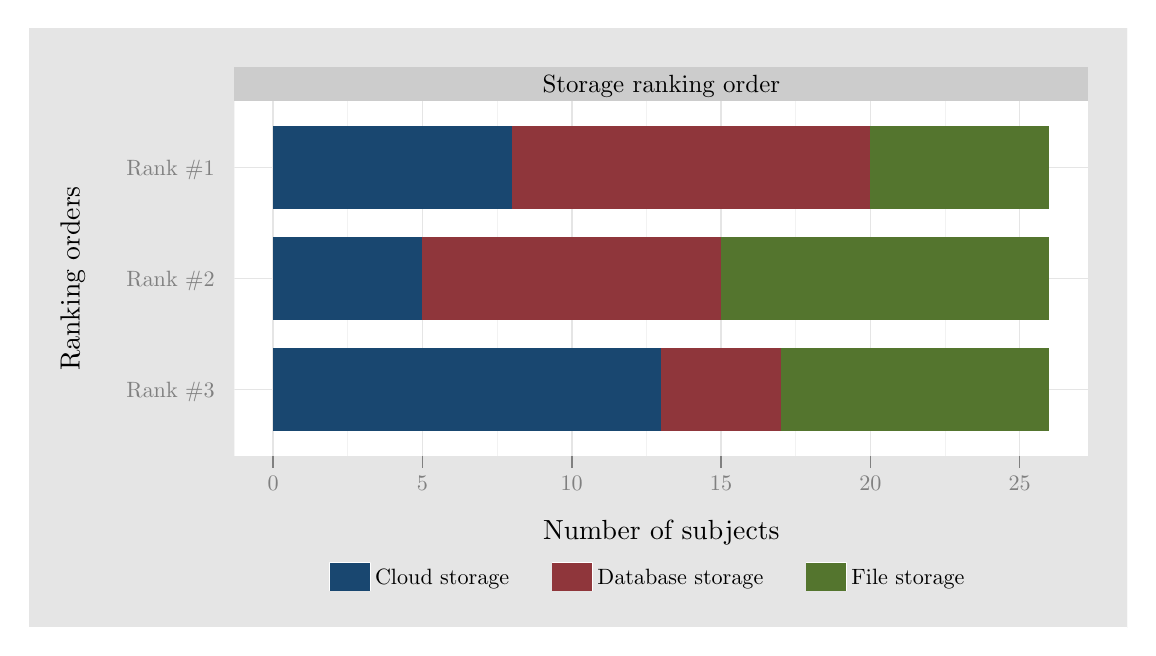
\begin{tikzpicture}[x=1pt,y=1pt]
\definecolor[named]{fillColor}{rgb}{1.00,1.00,1.00}
\path[use as bounding box,fill=fillColor,fill opacity=0.00] (0,0) rectangle (397.48,216.81);
\begin{scope}
\path[clip] (  0.00,  0.00) rectangle (397.48,216.81);
\definecolor[named]{drawColor}{rgb}{1.00,1.00,1.00}
\definecolor[named]{fillColor}{rgb}{0.90,0.90,0.90}

\path[draw=drawColor,line width= 0.6pt,line join=round,line cap=round,fill=fillColor] (  0.00,  0.00) rectangle (397.48,216.81);
\end{scope}
\begin{scope}
\path[clip] ( 74.67, 62.05) rectangle (383.26,190.36);
\definecolor[named]{fillColor}{rgb}{1.00,1.00,1.00}

\path[fill=fillColor] ( 74.67, 62.05) rectangle (383.26,190.36);
\definecolor[named]{drawColor}{rgb}{0.95,0.95,0.95}

\path[draw=drawColor,line width= 0.3pt,line join=round] (115.67, 62.05) --
	(115.67,190.36);

\path[draw=drawColor,line width= 0.3pt,line join=round] (169.62, 62.05) --
	(169.62,190.36);

\path[draw=drawColor,line width= 0.3pt,line join=round] (223.57, 62.05) --
	(223.57,190.36);

\path[draw=drawColor,line width= 0.3pt,line join=round] (277.52, 62.05) --
	(277.52,190.36);

\path[draw=drawColor,line width= 0.3pt,line join=round] (331.47, 62.05) --
	(331.47,190.36);
\definecolor[named]{drawColor}{rgb}{0.90,0.90,0.90}

\path[draw=drawColor,line width= 0.6pt,line join=round] ( 74.67, 86.11) --
	(383.26, 86.11);

\path[draw=drawColor,line width= 0.6pt,line join=round] ( 74.67,126.20) --
	(383.26,126.20);

\path[draw=drawColor,line width= 0.6pt,line join=round] ( 74.67,166.30) --
	(383.26,166.30);

\path[draw=drawColor,line width= 0.6pt,line join=round] ( 88.69, 62.05) --
	( 88.69,190.36);

\path[draw=drawColor,line width= 0.6pt,line join=round] (142.64, 62.05) --
	(142.64,190.36);

\path[draw=drawColor,line width= 0.6pt,line join=round] (196.59, 62.05) --
	(196.59,190.36);

\path[draw=drawColor,line width= 0.6pt,line join=round] (250.54, 62.05) --
	(250.54,190.36);

\path[draw=drawColor,line width= 0.6pt,line join=round] (304.49, 62.05) --
	(304.49,190.36);

\path[draw=drawColor,line width= 0.6pt,line join=round] (358.44, 62.05) --
	(358.44,190.36);
\definecolor[named]{fillColor}{rgb}{0.10,0.28,0.44}

\path[fill=fillColor] ( 88.69, 71.07) rectangle (228.96,101.14);
\definecolor[named]{fillColor}{rgb}{0.56,0.21,0.23}

\path[fill=fillColor] (228.96, 71.07) rectangle (272.12,101.14);
\definecolor[named]{fillColor}{rgb}{0.33,0.46,0.18}

\path[fill=fillColor] (272.12, 71.07) rectangle (369.23,101.14);
\definecolor[named]{fillColor}{rgb}{0.10,0.28,0.44}

\path[fill=fillColor] ( 88.69,111.17) rectangle (142.64,141.24);
\definecolor[named]{fillColor}{rgb}{0.56,0.21,0.23}

\path[fill=fillColor] (142.64,111.17) rectangle (250.54,141.24);
\definecolor[named]{fillColor}{rgb}{0.33,0.46,0.18}

\path[fill=fillColor] (250.54,111.17) rectangle (369.23,141.24);
\definecolor[named]{fillColor}{rgb}{0.10,0.28,0.44}

\path[fill=fillColor] ( 88.69,151.27) rectangle (175.01,181.34);
\definecolor[named]{fillColor}{rgb}{0.56,0.21,0.23}

\path[fill=fillColor] (175.01,151.27) rectangle (304.49,181.34);
\definecolor[named]{fillColor}{rgb}{0.33,0.46,0.18}

\path[fill=fillColor] (304.49,151.27) rectangle (369.23,181.34);
\end{scope}
\begin{scope}
\path[clip] (  0.00,  0.00) rectangle (397.48,216.81);
\definecolor[named]{fillColor}{rgb}{0.80,0.80,0.80}

\path[fill=fillColor] ( 74.67,190.36) rectangle (383.26,202.58);
\definecolor[named]{drawColor}{rgb}{0.00,0.00,0.00}

\node[text=drawColor,anchor=base,inner sep=0pt, outer sep=0pt, scale=  0.90] at (228.96,193.37) {Storage ranking order};
\end{scope}
\begin{scope}
\path[clip] (  0.00,  0.00) rectangle (397.48,216.81);
\definecolor[named]{drawColor}{rgb}{0.50,0.50,0.50}

\node[text=drawColor,anchor=base east,inner sep=0pt, outer sep=0pt, scale=  0.80] at ( 67.55, 83.35) {Rank \#3};

\node[text=drawColor,anchor=base east,inner sep=0pt, outer sep=0pt, scale=  0.80] at ( 67.55,123.45) {Rank \#2};

\node[text=drawColor,anchor=base east,inner sep=0pt, outer sep=0pt, scale=  0.80] at ( 67.55,163.55) {Rank \#1};
\end{scope}
\begin{scope}
\path[clip] (  0.00,  0.00) rectangle (397.48,216.81);
\definecolor[named]{drawColor}{rgb}{0.50,0.50,0.50}

\path[draw=drawColor,line width= 0.6pt,line join=round] ( 88.69, 57.78) --
	( 88.69, 62.05);

\path[draw=drawColor,line width= 0.6pt,line join=round] (142.64, 57.78) --
	(142.64, 62.05);

\path[draw=drawColor,line width= 0.6pt,line join=round] (196.59, 57.78) --
	(196.59, 62.05);

\path[draw=drawColor,line width= 0.6pt,line join=round] (250.54, 57.78) --
	(250.54, 62.05);

\path[draw=drawColor,line width= 0.6pt,line join=round] (304.49, 57.78) --
	(304.49, 62.05);

\path[draw=drawColor,line width= 0.6pt,line join=round] (358.44, 57.78) --
	(358.44, 62.05);
\end{scope}
\begin{scope}
\path[clip] (  0.00,  0.00) rectangle (397.48,216.81);
\definecolor[named]{drawColor}{rgb}{0.50,0.50,0.50}

\node[text=drawColor,anchor=base,inner sep=0pt, outer sep=0pt, scale=  0.80] at ( 88.69, 49.42) {0};

\node[text=drawColor,anchor=base,inner sep=0pt, outer sep=0pt, scale=  0.80] at (142.64, 49.42) {5};

\node[text=drawColor,anchor=base,inner sep=0pt, outer sep=0pt, scale=  0.80] at (196.59, 49.42) {10};

\node[text=drawColor,anchor=base,inner sep=0pt, outer sep=0pt, scale=  0.80] at (250.54, 49.42) {15};

\node[text=drawColor,anchor=base,inner sep=0pt, outer sep=0pt, scale=  0.80] at (304.49, 49.42) {20};

\node[text=drawColor,anchor=base,inner sep=0pt, outer sep=0pt, scale=  0.80] at (358.44, 49.42) {25};
\end{scope}
\begin{scope}
\path[clip] (  0.00,  0.00) rectangle (397.48,216.81);
\definecolor[named]{drawColor}{rgb}{0.00,0.00,0.00}

\node[text=drawColor,anchor=base,inner sep=0pt, outer sep=0pt, scale=  1.00] at (228.96, 31.70) {Number of subjects};
\end{scope}
\begin{scope}
\path[clip] (  0.00,  0.00) rectangle (397.48,216.81);
\definecolor[named]{drawColor}{rgb}{0.00,0.00,0.00}

\node[text=drawColor,rotate= 90.00,anchor=base,inner sep=0pt, outer sep=0pt, scale=  1.00] at ( 18.80,126.20) {Ranking orders};
\end{scope}
\begin{scope}
\path[clip] (  0.00,  0.00) rectangle (397.48,216.81);
\definecolor[named]{fillColor}{rgb}{0.90,0.90,0.90}

\path[fill=fillColor] (101.36,  9.15) rectangle (356.56, 27.65);
\end{scope}
\begin{scope}
\path[clip] (  0.00,  0.00) rectangle (397.48,216.81);
\definecolor[named]{drawColor}{rgb}{1.00,1.00,1.00}
\definecolor[named]{fillColor}{rgb}{1.00,1.00,1.00}

\path[draw=drawColor,line width= 0.6pt,line join=round,line cap=round,fill=fillColor] (109.25, 13.42) rectangle (123.70, 23.38);
\end{scope}
\begin{scope}
\path[clip] (  0.00,  0.00) rectangle (397.48,216.81);
\definecolor[named]{fillColor}{rgb}{0.10,0.28,0.44}

\path[fill=fillColor] (109.25, 13.42) rectangle (123.70, 23.38);

\path[] (109.25, 13.42) --
	(123.70, 23.38);
\end{scope}
\begin{scope}
\path[clip] (  0.00,  0.00) rectangle (397.48,216.81);
\definecolor[named]{drawColor}{rgb}{1.00,1.00,1.00}
\definecolor[named]{fillColor}{rgb}{1.00,1.00,1.00}

\path[draw=drawColor,line width= 0.6pt,line join=round,line cap=round,fill=fillColor] (189.59, 13.42) rectangle (204.04, 23.38);
\end{scope}
\begin{scope}
\path[clip] (  0.00,  0.00) rectangle (397.48,216.81);
\definecolor[named]{fillColor}{rgb}{0.56,0.21,0.23}

\path[fill=fillColor] (189.59, 13.42) rectangle (204.04, 23.38);

\path[] (189.59, 13.42) --
	(204.04, 23.38);
\end{scope}
\begin{scope}
\path[clip] (  0.00,  0.00) rectangle (397.48,216.81);
\definecolor[named]{drawColor}{rgb}{1.00,1.00,1.00}
\definecolor[named]{fillColor}{rgb}{1.00,1.00,1.00}

\path[draw=drawColor,line width= 0.6pt,line join=round,line cap=round,fill=fillColor] (281.42, 13.42) rectangle (295.87, 23.38);
\end{scope}
\begin{scope}
\path[clip] (  0.00,  0.00) rectangle (397.48,216.81);
\definecolor[named]{fillColor}{rgb}{0.33,0.46,0.18}

\path[fill=fillColor] (281.42, 13.42) rectangle (295.87, 23.38);

\path[] (281.42, 13.42) --
	(295.87, 23.38);
\end{scope}
\begin{scope}
\path[clip] (  0.00,  0.00) rectangle (397.48,216.81);
\definecolor[named]{drawColor}{rgb}{0.00,0.00,0.00}

\node[text=drawColor,anchor=base west,inner sep=0pt, outer sep=0pt, scale=  0.80] at (125.51, 15.64) {Cloud storage $\;\;\;\;\;$};
\end{scope}
\begin{scope}
\path[clip] (  0.00,  0.00) rectangle (397.48,216.81);
\definecolor[named]{drawColor}{rgb}{0.00,0.00,0.00}

\node[text=drawColor,anchor=base west,inner sep=0pt, outer sep=0pt, scale=  0.80] at (205.85, 15.64) {Database storage $\;\;\;\;\;$};
\end{scope}
\begin{scope}
\path[clip] (  0.00,  0.00) rectangle (397.48,216.81);
\definecolor[named]{drawColor}{rgb}{0.00,0.00,0.00}

\node[text=drawColor,anchor=base west,inner sep=0pt, outer sep=0pt, scale=  0.80] at (297.68, 15.64) {File storage $\;\;\;\;\;$};
\end{scope}
\end{tikzpicture}

 }
 \caption[Survey participants' rankings of storage solutions]{Survey participants' rankings of data storage solutions.}
 \label{fig:experimentation:survey:storage-solutions-ranking}
\end{figure}

%%%\subsubsection{Repository Simplicity}
%%%\label{sec:evaluation:developer-survey:results:simplicity}

\begin{figure}
 \centering
 \framebox[\textwidth]{
 % Created by tikzDevice version 0.6.2-92-0ad2792 on 2013-04-07 23:43:57
% !TEX encoding = UTF-8 Unicode
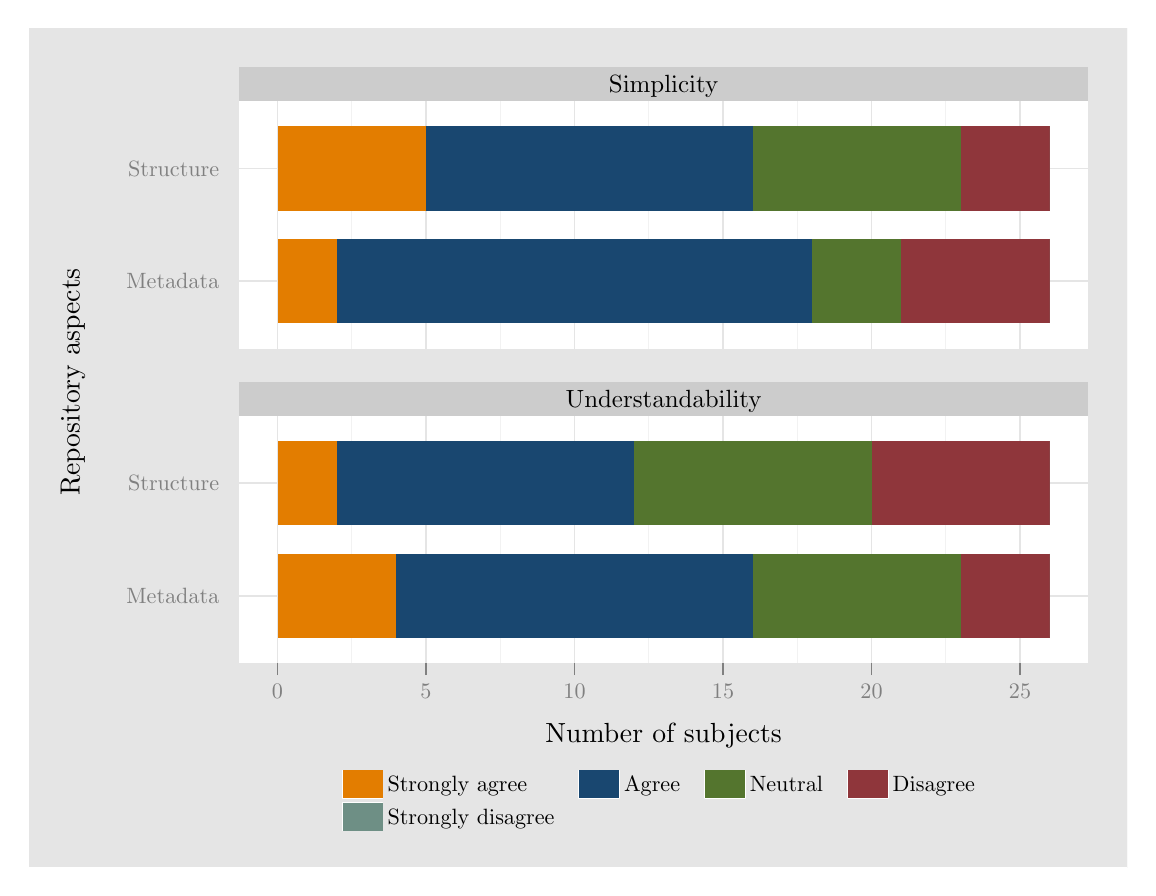
\begin{tikzpicture}[x=1pt,y=1pt]
\definecolor[named]{fillColor}{rgb}{1.00,1.00,1.00}
\path[use as bounding box,fill=fillColor,fill opacity=0.00] (0,0) rectangle (397.48,303.53);
\begin{scope}
\path[clip] (  0.00,  0.00) rectangle (397.48,303.53);
\definecolor[named]{drawColor}{rgb}{1.00,1.00,1.00}
\definecolor[named]{fillColor}{rgb}{0.90,0.90,0.90}

\path[draw=drawColor,line width= 0.6pt,line join=round,line cap=round,fill=fillColor] (  0.00,  0.00) rectangle (397.48,303.53);
\end{scope}
\begin{scope}
\path[clip] ( 76.33,187.58) rectangle (383.26,277.09);
\definecolor[named]{fillColor}{rgb}{1.00,1.00,1.00}

\path[fill=fillColor] ( 76.33,187.58) rectangle (383.26,277.09);
\definecolor[named]{drawColor}{rgb}{0.95,0.95,0.95}

\path[draw=drawColor,line width= 0.3pt,line join=round] (117.11,187.58) --
	(117.11,277.09);

\path[draw=drawColor,line width= 0.3pt,line join=round] (170.77,187.58) --
	(170.77,277.09);

\path[draw=drawColor,line width= 0.3pt,line join=round] (224.43,187.58) --
	(224.43,277.09);

\path[draw=drawColor,line width= 0.3pt,line join=round] (278.09,187.58) --
	(278.09,277.09);

\path[draw=drawColor,line width= 0.3pt,line join=round] (331.75,187.58) --
	(331.75,277.09);
\definecolor[named]{drawColor}{rgb}{0.90,0.90,0.90}

\path[draw=drawColor,line width= 0.6pt,line join=round] ( 76.33,211.99) --
	(383.26,211.99);

\path[draw=drawColor,line width= 0.6pt,line join=round] ( 76.33,252.68) --
	(383.26,252.68);

\path[draw=drawColor,line width= 0.6pt,line join=round] ( 90.28,187.58) --
	( 90.28,277.09);

\path[draw=drawColor,line width= 0.6pt,line join=round] (143.94,187.58) --
	(143.94,277.09);

\path[draw=drawColor,line width= 0.6pt,line join=round] (197.60,187.58) --
	(197.60,277.09);

\path[draw=drawColor,line width= 0.6pt,line join=round] (251.26,187.58) --
	(251.26,277.09);

\path[draw=drawColor,line width= 0.6pt,line join=round] (304.92,187.58) --
	(304.92,277.09);

\path[draw=drawColor,line width= 0.6pt,line join=round] (358.58,187.58) --
	(358.58,277.09);
\definecolor[named]{fillColor}{rgb}{0.89,0.49,0.00}

\path[fill=fillColor] ( 90.28,196.74) rectangle (111.75,227.25);
\definecolor[named]{fillColor}{rgb}{0.10,0.28,0.44}

\path[fill=fillColor] (111.75,196.74) rectangle (283.45,227.25);
\definecolor[named]{fillColor}{rgb}{0.33,0.46,0.18}

\path[fill=fillColor] (283.45,196.74) rectangle (315.65,227.25);
\definecolor[named]{fillColor}{rgb}{0.56,0.21,0.23}

\path[fill=fillColor] (315.65,196.74) rectangle (369.31,227.25);
\definecolor[named]{fillColor}{rgb}{0.43,0.56,0.52}

\path[fill=fillColor] (369.31,196.74) rectangle (369.31,227.25);
\definecolor[named]{fillColor}{rgb}{0.89,0.49,0.00}

\path[fill=fillColor] ( 90.28,237.42) rectangle (143.94,267.93);
\definecolor[named]{fillColor}{rgb}{0.10,0.28,0.44}

\path[fill=fillColor] (143.94,237.42) rectangle (261.99,267.93);
\definecolor[named]{fillColor}{rgb}{0.33,0.46,0.18}

\path[fill=fillColor] (261.99,237.42) rectangle (337.11,267.93);
\definecolor[named]{fillColor}{rgb}{0.56,0.21,0.23}

\path[fill=fillColor] (337.11,237.42) rectangle (369.31,267.93);
\definecolor[named]{fillColor}{rgb}{0.43,0.56,0.52}

\path[fill=fillColor] (369.31,237.42) rectangle (369.31,267.93);
\end{scope}
\begin{scope}
\path[clip] ( 76.33, 73.81) rectangle (383.26,163.32);
\definecolor[named]{fillColor}{rgb}{1.00,1.00,1.00}

\path[fill=fillColor] ( 76.33, 73.81) rectangle (383.26,163.32);
\definecolor[named]{drawColor}{rgb}{0.95,0.95,0.95}

\path[draw=drawColor,line width= 0.3pt,line join=round] (117.11, 73.81) --
	(117.11,163.32);

\path[draw=drawColor,line width= 0.3pt,line join=round] (170.77, 73.81) --
	(170.77,163.32);

\path[draw=drawColor,line width= 0.3pt,line join=round] (224.43, 73.81) --
	(224.43,163.32);

\path[draw=drawColor,line width= 0.3pt,line join=round] (278.09, 73.81) --
	(278.09,163.32);

\path[draw=drawColor,line width= 0.3pt,line join=round] (331.75, 73.81) --
	(331.75,163.32);
\definecolor[named]{drawColor}{rgb}{0.90,0.90,0.90}

\path[draw=drawColor,line width= 0.6pt,line join=round] ( 76.33, 98.22) --
	(383.26, 98.22);

\path[draw=drawColor,line width= 0.6pt,line join=round] ( 76.33,138.91) --
	(383.26,138.91);

\path[draw=drawColor,line width= 0.6pt,line join=round] ( 90.28, 73.81) --
	( 90.28,163.32);

\path[draw=drawColor,line width= 0.6pt,line join=round] (143.94, 73.81) --
	(143.94,163.32);

\path[draw=drawColor,line width= 0.6pt,line join=round] (197.60, 73.81) --
	(197.60,163.32);

\path[draw=drawColor,line width= 0.6pt,line join=round] (251.26, 73.81) --
	(251.26,163.32);

\path[draw=drawColor,line width= 0.6pt,line join=round] (304.92, 73.81) --
	(304.92,163.32);

\path[draw=drawColor,line width= 0.6pt,line join=round] (358.58, 73.81) --
	(358.58,163.32);
\definecolor[named]{fillColor}{rgb}{0.89,0.49,0.00}

\path[fill=fillColor] ( 90.28, 82.97) rectangle (133.21,113.48);
\definecolor[named]{fillColor}{rgb}{0.10,0.28,0.44}

\path[fill=fillColor] (133.21, 82.97) rectangle (261.99,113.48);
\definecolor[named]{fillColor}{rgb}{0.33,0.46,0.18}

\path[fill=fillColor] (261.99, 82.97) rectangle (337.11,113.48);
\definecolor[named]{fillColor}{rgb}{0.56,0.21,0.23}

\path[fill=fillColor] (337.11, 82.97) rectangle (369.31,113.48);
\definecolor[named]{fillColor}{rgb}{0.43,0.56,0.52}

\path[fill=fillColor] (369.31, 82.97) rectangle (369.31,113.48);
\definecolor[named]{fillColor}{rgb}{0.89,0.49,0.00}

\path[fill=fillColor] ( 90.28,123.65) rectangle (111.75,154.16);
\definecolor[named]{fillColor}{rgb}{0.10,0.28,0.44}

\path[fill=fillColor] (111.75,123.65) rectangle (219.06,154.16);
\definecolor[named]{fillColor}{rgb}{0.33,0.46,0.18}

\path[fill=fillColor] (219.06,123.65) rectangle (304.92,154.16);
\definecolor[named]{fillColor}{rgb}{0.56,0.21,0.23}

\path[fill=fillColor] (304.92,123.65) rectangle (369.31,154.16);
\definecolor[named]{fillColor}{rgb}{0.43,0.56,0.52}

\path[fill=fillColor] (369.31,123.65) rectangle (369.31,154.16);
\end{scope}
\begin{scope}
\path[clip] (  0.00,  0.00) rectangle (397.48,303.53);
\definecolor[named]{fillColor}{rgb}{0.80,0.80,0.80}

\path[fill=fillColor] ( 76.33,277.09) rectangle (383.26,289.31);
\definecolor[named]{drawColor}{rgb}{0.00,0.00,0.00}

\node[text=drawColor,anchor=base,inner sep=0pt, outer sep=0pt, scale=  0.90] at (229.80,280.10) {Simplicity};
\end{scope}
\begin{scope}
\path[clip] (  0.00,  0.00) rectangle (397.48,303.53);
\definecolor[named]{fillColor}{rgb}{0.80,0.80,0.80}

\path[fill=fillColor] ( 76.33,163.32) rectangle (383.26,175.54);
\definecolor[named]{drawColor}{rgb}{0.00,0.00,0.00}

\node[text=drawColor,anchor=base,inner sep=0pt, outer sep=0pt, scale=  0.90] at (229.80,166.33) {Understandability};
\end{scope}
\begin{scope}
\path[clip] (  0.00,  0.00) rectangle (397.48,303.53);
\definecolor[named]{drawColor}{rgb}{0.50,0.50,0.50}

\node[text=drawColor,anchor=base east,inner sep=0pt, outer sep=0pt, scale=  0.80] at ( 69.22,209.24) {Metadata};

\node[text=drawColor,anchor=base east,inner sep=0pt, outer sep=0pt, scale=  0.80] at ( 69.22,249.92) {Structure};
\end{scope}
\begin{scope}
\path[clip] (  0.00,  0.00) rectangle (397.48,303.53);
\definecolor[named]{drawColor}{rgb}{0.50,0.50,0.50}

\node[text=drawColor,anchor=base east,inner sep=0pt, outer sep=0pt, scale=  0.80] at ( 69.22, 95.47) {Metadata};

\node[text=drawColor,anchor=base east,inner sep=0pt, outer sep=0pt, scale=  0.80] at ( 69.22,136.15) {Structure};
\end{scope}
\begin{scope}
\path[clip] (  0.00,  0.00) rectangle (397.48,303.53);
\definecolor[named]{drawColor}{rgb}{0.50,0.50,0.50}

\path[draw=drawColor,line width= 0.6pt,line join=round] ( 90.28, 69.54) --
	( 90.28, 73.81);

\path[draw=drawColor,line width= 0.6pt,line join=round] (143.94, 69.54) --
	(143.94, 73.81);

\path[draw=drawColor,line width= 0.6pt,line join=round] (197.60, 69.54) --
	(197.60, 73.81);

\path[draw=drawColor,line width= 0.6pt,line join=round] (251.26, 69.54) --
	(251.26, 73.81);

\path[draw=drawColor,line width= 0.6pt,line join=round] (304.92, 69.54) --
	(304.92, 73.81);

\path[draw=drawColor,line width= 0.6pt,line join=round] (358.58, 69.54) --
	(358.58, 73.81);
\end{scope}
\begin{scope}
\path[clip] (  0.00,  0.00) rectangle (397.48,303.53);
\definecolor[named]{drawColor}{rgb}{0.50,0.50,0.50}

\node[text=drawColor,anchor=base,inner sep=0pt, outer sep=0pt, scale=  0.80] at ( 90.28, 61.19) {0};

\node[text=drawColor,anchor=base,inner sep=0pt, outer sep=0pt, scale=  0.80] at (143.94, 61.19) {5};

\node[text=drawColor,anchor=base,inner sep=0pt, outer sep=0pt, scale=  0.80] at (197.60, 61.19) {10};

\node[text=drawColor,anchor=base,inner sep=0pt, outer sep=0pt, scale=  0.80] at (251.26, 61.19) {15};

\node[text=drawColor,anchor=base,inner sep=0pt, outer sep=0pt, scale=  0.80] at (304.92, 61.19) {20};

\node[text=drawColor,anchor=base,inner sep=0pt, outer sep=0pt, scale=  0.80] at (358.58, 61.19) {25};
\end{scope}
\begin{scope}
\path[clip] (  0.00,  0.00) rectangle (397.48,303.53);
\definecolor[named]{drawColor}{rgb}{0.00,0.00,0.00}

\node[text=drawColor,anchor=base,inner sep=0pt, outer sep=0pt, scale=  1.00] at (229.80, 45.27) {Number of subjects};
\end{scope}
\begin{scope}
\path[clip] (  0.00,  0.00) rectangle (397.48,303.53);
\definecolor[named]{drawColor}{rgb}{0.00,0.00,0.00}

\node[text=drawColor,rotate= 90.00,anchor=base,inner sep=0pt, outer sep=0pt, scale=  1.00] at ( 18.80,175.45) {Repository aspects};
\end{scope}
\begin{scope}
\path[clip] (  0.00,  0.00) rectangle (397.48,303.53);
\definecolor[named]{fillColor}{rgb}{0.90,0.90,0.90}

\path[fill=fillColor] (105.91,  9.15) rectangle (353.68, 39.41);
\end{scope}
\begin{scope}
\path[clip] (  0.00,  0.00) rectangle (397.48,303.53);
\definecolor[named]{drawColor}{rgb}{1.00,1.00,1.00}
\definecolor[named]{fillColor}{rgb}{1.00,1.00,1.00}

\path[draw=drawColor,line width= 0.6pt,line join=round,line cap=round,fill=fillColor] (113.79, 25.19) rectangle (128.24, 35.14);
\end{scope}
\begin{scope}
\path[clip] (  0.00,  0.00) rectangle (397.48,303.53);
\definecolor[named]{fillColor}{rgb}{0.89,0.49,0.00}

\path[fill=fillColor] (113.79, 25.19) rectangle (128.24, 35.14);

\path[] (113.79, 25.19) --
	(128.24, 35.14);
\end{scope}
\begin{scope}
\path[clip] (  0.00,  0.00) rectangle (397.48,303.53);
\definecolor[named]{drawColor}{rgb}{1.00,1.00,1.00}
\definecolor[named]{fillColor}{rgb}{1.00,1.00,1.00}

\path[draw=drawColor,line width= 0.6pt,line join=round,line cap=round,fill=fillColor] (199.26, 25.19) rectangle (213.72, 35.14);
\end{scope}
\begin{scope}
\path[clip] (  0.00,  0.00) rectangle (397.48,303.53);
\definecolor[named]{fillColor}{rgb}{0.10,0.28,0.44}

\path[fill=fillColor] (199.26, 25.19) rectangle (213.72, 35.14);

\path[] (199.26, 25.19) --
	(213.72, 35.14);
\end{scope}
\begin{scope}
\path[clip] (  0.00,  0.00) rectangle (397.48,303.53);
\definecolor[named]{drawColor}{rgb}{1.00,1.00,1.00}
\definecolor[named]{fillColor}{rgb}{1.00,1.00,1.00}

\path[draw=drawColor,line width= 0.6pt,line join=round,line cap=round,fill=fillColor] (244.68, 25.19) rectangle (259.13, 35.14);
\end{scope}
\begin{scope}
\path[clip] (  0.00,  0.00) rectangle (397.48,303.53);
\definecolor[named]{fillColor}{rgb}{0.33,0.46,0.18}

\path[fill=fillColor] (244.68, 25.19) rectangle (259.13, 35.14);

\path[] (244.68, 25.19) --
	(259.13, 35.14);
\end{scope}
\begin{scope}
\path[clip] (  0.00,  0.00) rectangle (397.48,303.53);
\definecolor[named]{drawColor}{rgb}{1.00,1.00,1.00}
\definecolor[named]{fillColor}{rgb}{1.00,1.00,1.00}

\path[draw=drawColor,line width= 0.6pt,line join=round,line cap=round,fill=fillColor] (296.32, 25.19) rectangle (310.77, 35.14);
\end{scope}
\begin{scope}
\path[clip] (  0.00,  0.00) rectangle (397.48,303.53);
\definecolor[named]{fillColor}{rgb}{0.56,0.21,0.23}

\path[fill=fillColor] (296.32, 25.19) rectangle (310.77, 35.14);

\path[] (296.32, 25.19) --
	(310.77, 35.14);
\end{scope}
\begin{scope}
\path[clip] (  0.00,  0.00) rectangle (397.48,303.53);
\definecolor[named]{drawColor}{rgb}{1.00,1.00,1.00}
\definecolor[named]{fillColor}{rgb}{1.00,1.00,1.00}

\path[draw=drawColor,line width= 0.6pt,line join=round,line cap=round,fill=fillColor] (113.79, 13.42) rectangle (128.24, 23.38);
\end{scope}
\begin{scope}
\path[clip] (  0.00,  0.00) rectangle (397.48,303.53);
\definecolor[named]{fillColor}{rgb}{0.43,0.56,0.52}

\path[fill=fillColor] (113.79, 13.42) rectangle (128.24, 23.38);

\path[] (113.79, 13.42) --
	(128.24, 23.38);
\end{scope}
\begin{scope}
\path[clip] (  0.00,  0.00) rectangle (397.48,303.53);
\definecolor[named]{drawColor}{rgb}{0.00,0.00,0.00}

\node[text=drawColor,anchor=base west,inner sep=0pt, outer sep=0pt, scale=  0.80] at (130.05, 27.41) {Strongly agree $\;\;$};
\end{scope}
\begin{scope}
\path[clip] (  0.00,  0.00) rectangle (397.48,303.53);
\definecolor[named]{drawColor}{rgb}{0.00,0.00,0.00}

\node[text=drawColor,anchor=base west,inner sep=0pt, outer sep=0pt, scale=  0.80] at (215.52, 27.41) {Agree $\;\;$};
\end{scope}
\begin{scope}
\path[clip] (  0.00,  0.00) rectangle (397.48,303.53);
\definecolor[named]{drawColor}{rgb}{0.00,0.00,0.00}

\node[text=drawColor,anchor=base west,inner sep=0pt, outer sep=0pt, scale=  0.80] at (260.94, 27.41) {Neutral $\;\;$};
\end{scope}
\begin{scope}
\path[clip] (  0.00,  0.00) rectangle (397.48,303.53);
\definecolor[named]{drawColor}{rgb}{0.00,0.00,0.00}

\node[text=drawColor,anchor=base west,inner sep=0pt, outer sep=0pt, scale=  0.80] at (312.58, 27.41) {Disagree $\;\;$};
\end{scope}
\begin{scope}
\path[clip] (  0.00,  0.00) rectangle (397.48,303.53);
\definecolor[named]{drawColor}{rgb}{0.00,0.00,0.00}

\node[text=drawColor,anchor=base west,inner sep=0pt, outer sep=0pt, scale=  0.80] at (130.05, 15.64) {Strongly disagree $\;\;$};
\end{scope}
\end{tikzpicture}

 }
 \caption[Survey participants' simplicity\& understandability ratings]{Survey participants' simplicity and understandability ratings of repository design.}
 \label{fig:experimentation:survey:simplicity-understandability}
\end{figure}

\begin{figure}
 \centering
 \framebox[\textwidth]{
 % Created by tikzDevice version 0.6.2-92-0ad2792 on 2013-04-07 23:44:31
% !TEX encoding = UTF-8 Unicode
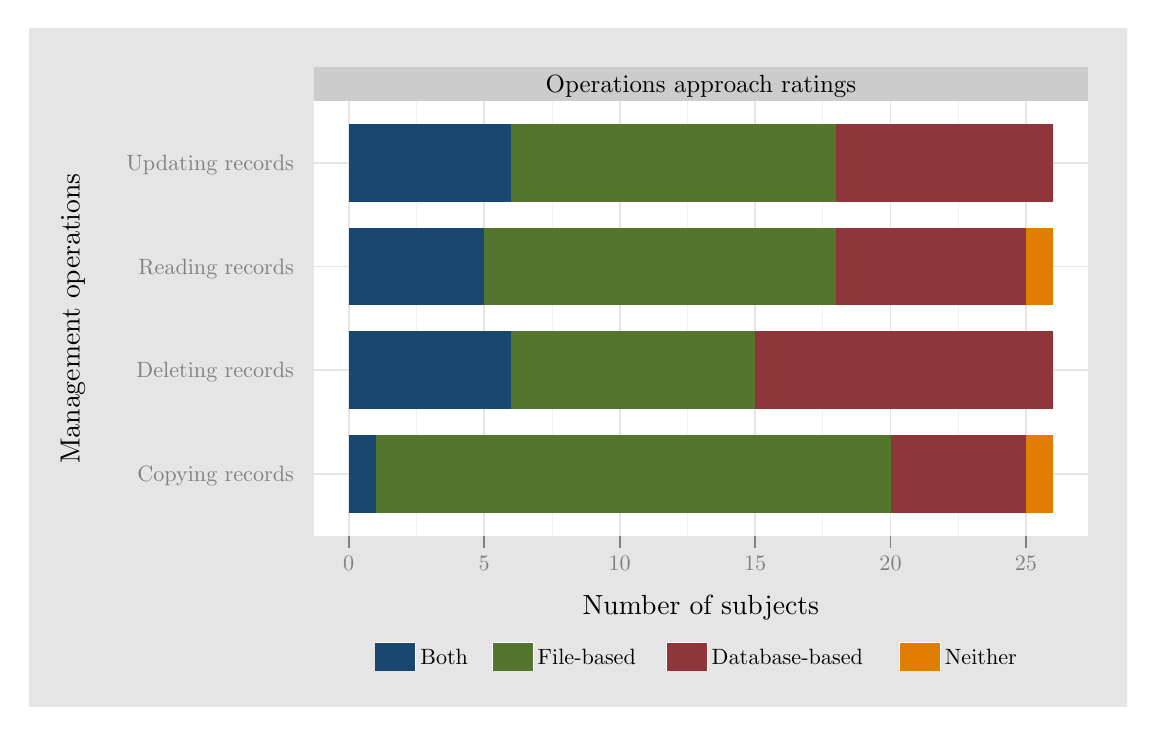
\begin{tikzpicture}[x=1pt,y=1pt]
\definecolor[named]{fillColor}{rgb}{1.00,1.00,1.00}
\path[use as bounding box,fill=fillColor,fill opacity=0.00] (0,0) rectangle (397.48,245.72);
\begin{scope}
\path[clip] (  0.00,  0.00) rectangle (397.48,245.72);
\definecolor[named]{drawColor}{rgb}{1.00,1.00,1.00}
\definecolor[named]{fillColor}{rgb}{0.90,0.90,0.90}

\path[draw=drawColor,line width= 0.6pt,line join=round,line cap=round,fill=fillColor] (  0.00,  0.00) rectangle (397.48,245.72);
\end{scope}
\begin{scope}
\path[clip] (103.30, 62.05) rectangle (383.26,219.27);
\definecolor[named]{fillColor}{rgb}{1.00,1.00,1.00}

\path[fill=fillColor] (103.30, 62.05) rectangle (383.26,219.27);
\definecolor[named]{drawColor}{rgb}{0.95,0.95,0.95}

\path[draw=drawColor,line width= 0.3pt,line join=round] (140.50, 62.05) --
	(140.50,219.27);

\path[draw=drawColor,line width= 0.3pt,line join=round] (189.44, 62.05) --
	(189.44,219.27);

\path[draw=drawColor,line width= 0.3pt,line join=round] (238.39, 62.05) --
	(238.39,219.27);

\path[draw=drawColor,line width= 0.3pt,line join=round] (287.33, 62.05) --
	(287.33,219.27);

\path[draw=drawColor,line width= 0.3pt,line join=round] (336.27, 62.05) --
	(336.27,219.27);
\definecolor[named]{drawColor}{rgb}{0.90,0.90,0.90}

\path[draw=drawColor,line width= 0.6pt,line join=round] (103.30, 84.51) --
	(383.26, 84.51);

\path[draw=drawColor,line width= 0.6pt,line join=round] (103.30,121.94) --
	(383.26,121.94);

\path[draw=drawColor,line width= 0.6pt,line join=round] (103.30,159.38) --
	(383.26,159.38);

\path[draw=drawColor,line width= 0.6pt,line join=round] (103.30,196.81) --
	(383.26,196.81);

\path[draw=drawColor,line width= 0.6pt,line join=round] (116.03, 62.05) --
	(116.03,219.27);

\path[draw=drawColor,line width= 0.6pt,line join=round] (164.97, 62.05) --
	(164.97,219.27);

\path[draw=drawColor,line width= 0.6pt,line join=round] (213.92, 62.05) --
	(213.92,219.27);

\path[draw=drawColor,line width= 0.6pt,line join=round] (262.86, 62.05) --
	(262.86,219.27);

\path[draw=drawColor,line width= 0.6pt,line join=round] (311.80, 62.05) --
	(311.80,219.27);

\path[draw=drawColor,line width= 0.6pt,line join=round] (360.74, 62.05) --
	(360.74,219.27);
\definecolor[named]{fillColor}{rgb}{0.10,0.28,0.44}

\path[fill=fillColor] (116.03, 70.47) rectangle (125.82, 98.55);
\definecolor[named]{fillColor}{rgb}{0.33,0.46,0.18}

\path[fill=fillColor] (125.82, 70.47) rectangle (311.80, 98.55);
\definecolor[named]{fillColor}{rgb}{0.56,0.21,0.23}

\path[fill=fillColor] (311.80, 70.47) rectangle (360.74, 98.55);
\definecolor[named]{fillColor}{rgb}{0.89,0.49,0.00}

\path[fill=fillColor] (360.74, 70.47) rectangle (370.53, 98.55);
\definecolor[named]{fillColor}{rgb}{0.10,0.28,0.44}

\path[fill=fillColor] (116.03,107.90) rectangle (174.76,135.98);
\definecolor[named]{fillColor}{rgb}{0.33,0.46,0.18}

\path[fill=fillColor] (174.76,107.90) rectangle (262.86,135.98);
\definecolor[named]{fillColor}{rgb}{0.56,0.21,0.23}

\path[fill=fillColor] (262.86,107.90) rectangle (370.53,135.98);
\definecolor[named]{fillColor}{rgb}{0.89,0.49,0.00}

\path[fill=fillColor] (370.53,107.90) rectangle (370.53,135.98);
\definecolor[named]{fillColor}{rgb}{0.10,0.28,0.44}

\path[fill=fillColor] (116.03,145.34) rectangle (164.97,173.41);
\definecolor[named]{fillColor}{rgb}{0.33,0.46,0.18}

\path[fill=fillColor] (164.97,145.34) rectangle (292.22,173.41);
\definecolor[named]{fillColor}{rgb}{0.56,0.21,0.23}

\path[fill=fillColor] (292.22,145.34) rectangle (360.74,173.41);
\definecolor[named]{fillColor}{rgb}{0.89,0.49,0.00}

\path[fill=fillColor] (360.74,145.34) rectangle (370.53,173.41);
\definecolor[named]{fillColor}{rgb}{0.10,0.28,0.44}

\path[fill=fillColor] (116.03,182.77) rectangle (174.76,210.85);
\definecolor[named]{fillColor}{rgb}{0.33,0.46,0.18}

\path[fill=fillColor] (174.76,182.77) rectangle (292.22,210.85);
\definecolor[named]{fillColor}{rgb}{0.56,0.21,0.23}

\path[fill=fillColor] (292.22,182.77) rectangle (370.53,210.85);
\definecolor[named]{fillColor}{rgb}{0.89,0.49,0.00}

\path[fill=fillColor] (370.53,182.77) rectangle (370.53,210.85);
\end{scope}
\begin{scope}
\path[clip] (  0.00,  0.00) rectangle (397.48,245.72);
\definecolor[named]{fillColor}{rgb}{0.80,0.80,0.80}

\path[fill=fillColor] (103.30,219.27) rectangle (383.26,231.49);
\definecolor[named]{drawColor}{rgb}{0.00,0.00,0.00}

\node[text=drawColor,anchor=base,inner sep=0pt, outer sep=0pt, scale=  0.90] at (243.28,222.28) {Operations approach ratings};
\end{scope}
\begin{scope}
\path[clip] (  0.00,  0.00) rectangle (397.48,245.72);
\definecolor[named]{drawColor}{rgb}{0.50,0.50,0.50}

\node[text=drawColor,anchor=base east,inner sep=0pt, outer sep=0pt, scale=  0.80] at ( 96.19, 81.75) {Copying records};

\node[text=drawColor,anchor=base east,inner sep=0pt, outer sep=0pt, scale=  0.80] at ( 96.19,119.19) {Deleting records};

\node[text=drawColor,anchor=base east,inner sep=0pt, outer sep=0pt, scale=  0.80] at ( 96.19,156.62) {Reading records};

\node[text=drawColor,anchor=base east,inner sep=0pt, outer sep=0pt, scale=  0.80] at ( 96.19,194.06) {Updating records};
\end{scope}
\begin{scope}
\path[clip] (  0.00,  0.00) rectangle (397.48,245.72);
\definecolor[named]{drawColor}{rgb}{0.50,0.50,0.50}

\path[draw=drawColor,line width= 0.6pt,line join=round] (116.03, 57.78) --
	(116.03, 62.05);

\path[draw=drawColor,line width= 0.6pt,line join=round] (164.97, 57.78) --
	(164.97, 62.05);

\path[draw=drawColor,line width= 0.6pt,line join=round] (213.92, 57.78) --
	(213.92, 62.05);

\path[draw=drawColor,line width= 0.6pt,line join=round] (262.86, 57.78) --
	(262.86, 62.05);

\path[draw=drawColor,line width= 0.6pt,line join=round] (311.80, 57.78) --
	(311.80, 62.05);

\path[draw=drawColor,line width= 0.6pt,line join=round] (360.74, 57.78) --
	(360.74, 62.05);
\end{scope}
\begin{scope}
\path[clip] (  0.00,  0.00) rectangle (397.48,245.72);
\definecolor[named]{drawColor}{rgb}{0.50,0.50,0.50}

\node[text=drawColor,anchor=base,inner sep=0pt, outer sep=0pt, scale=  0.80] at (116.03, 49.42) {0};

\node[text=drawColor,anchor=base,inner sep=0pt, outer sep=0pt, scale=  0.80] at (164.97, 49.42) {5};

\node[text=drawColor,anchor=base,inner sep=0pt, outer sep=0pt, scale=  0.80] at (213.92, 49.42) {10};

\node[text=drawColor,anchor=base,inner sep=0pt, outer sep=0pt, scale=  0.80] at (262.86, 49.42) {15};

\node[text=drawColor,anchor=base,inner sep=0pt, outer sep=0pt, scale=  0.80] at (311.80, 49.42) {20};

\node[text=drawColor,anchor=base,inner sep=0pt, outer sep=0pt, scale=  0.80] at (360.74, 49.42) {25};
\end{scope}
\begin{scope}
\path[clip] (  0.00,  0.00) rectangle (397.48,245.72);
\definecolor[named]{drawColor}{rgb}{0.00,0.00,0.00}

\node[text=drawColor,anchor=base,inner sep=0pt, outer sep=0pt, scale=  1.00] at (243.28, 33.50) {Number of subjects};
\end{scope}
\begin{scope}
\path[clip] (  0.00,  0.00) rectangle (397.48,245.72);
\definecolor[named]{drawColor}{rgb}{0.00,0.00,0.00}

\node[text=drawColor,rotate= 90.00,anchor=base,inner sep=0pt, outer sep=0pt, scale=  1.00] at ( 18.80,140.66) {Management operations};
\end{scope}
\begin{scope}
\path[clip] (  0.00,  0.00) rectangle (397.48,245.72);
\definecolor[named]{fillColor}{rgb}{0.90,0.90,0.90}

\path[fill=fillColor] (117.75,  9.15) rectangle (368.81, 27.65);
\end{scope}
\begin{scope}
\path[clip] (  0.00,  0.00) rectangle (397.48,245.72);
\definecolor[named]{drawColor}{rgb}{1.00,1.00,1.00}
\definecolor[named]{fillColor}{rgb}{1.00,1.00,1.00}

\path[draw=drawColor,line width= 0.6pt,line join=round,line cap=round,fill=fillColor] (125.63, 13.42) rectangle (140.08, 23.38);
\end{scope}
\begin{scope}
\path[clip] (  0.00,  0.00) rectangle (397.48,245.72);
\definecolor[named]{fillColor}{rgb}{0.10,0.28,0.44}

\path[fill=fillColor] (125.63, 13.42) rectangle (140.08, 23.38);

\path[] (125.63, 13.42) --
	(140.08, 23.38);
\end{scope}
\begin{scope}
\path[clip] (  0.00,  0.00) rectangle (397.48,245.72);
\definecolor[named]{drawColor}{rgb}{1.00,1.00,1.00}
\definecolor[named]{fillColor}{rgb}{1.00,1.00,1.00}

\path[draw=drawColor,line width= 0.6pt,line join=round,line cap=round,fill=fillColor] (168.03, 13.42) rectangle (182.48, 23.38);
\end{scope}
\begin{scope}
\path[clip] (  0.00,  0.00) rectangle (397.48,245.72);
\definecolor[named]{fillColor}{rgb}{0.33,0.46,0.18}

\path[fill=fillColor] (168.03, 13.42) rectangle (182.48, 23.38);

\path[] (168.03, 13.42) --
	(182.48, 23.38);
\end{scope}
\begin{scope}
\path[clip] (  0.00,  0.00) rectangle (397.48,245.72);
\definecolor[named]{drawColor}{rgb}{1.00,1.00,1.00}
\definecolor[named]{fillColor}{rgb}{1.00,1.00,1.00}

\path[draw=drawColor,line width= 0.6pt,line join=round,line cap=round,fill=fillColor] (230.91, 13.42) rectangle (245.36, 23.38);
\end{scope}
\begin{scope}
\path[clip] (  0.00,  0.00) rectangle (397.48,245.72);
\definecolor[named]{fillColor}{rgb}{0.56,0.21,0.23}

\path[fill=fillColor] (230.91, 13.42) rectangle (245.36, 23.38);

\path[] (230.91, 13.42) --
	(245.36, 23.38);
\end{scope}
\begin{scope}
\path[clip] (  0.00,  0.00) rectangle (397.48,245.72);
\definecolor[named]{drawColor}{rgb}{1.00,1.00,1.00}
\definecolor[named]{fillColor}{rgb}{1.00,1.00,1.00}

\path[draw=drawColor,line width= 0.6pt,line join=round,line cap=round,fill=fillColor] (315.16, 13.42) rectangle (329.61, 23.38);
\end{scope}
\begin{scope}
\path[clip] (  0.00,  0.00) rectangle (397.48,245.72);
\definecolor[named]{fillColor}{rgb}{0.89,0.49,0.00}

\path[fill=fillColor] (315.16, 13.42) rectangle (329.61, 23.38);

\path[] (315.16, 13.42) --
	(329.61, 23.38);
\end{scope}
\begin{scope}
\path[clip] (  0.00,  0.00) rectangle (397.48,245.72);
\definecolor[named]{drawColor}{rgb}{0.00,0.00,0.00}

\node[text=drawColor,anchor=base west,inner sep=0pt, outer sep=0pt, scale=  0.80] at (141.89, 15.64) {Both $\;\;$};
\end{scope}
\begin{scope}
\path[clip] (  0.00,  0.00) rectangle (397.48,245.72);
\definecolor[named]{drawColor}{rgb}{0.00,0.00,0.00}

\node[text=drawColor,anchor=base west,inner sep=0pt, outer sep=0pt, scale=  0.80] at (184.29, 15.64) {File-based $\;\;\;$};
\end{scope}
\begin{scope}
\path[clip] (  0.00,  0.00) rectangle (397.48,245.72);
\definecolor[named]{drawColor}{rgb}{0.00,0.00,0.00}

\node[text=drawColor,anchor=base west,inner sep=0pt, outer sep=0pt, scale=  0.80] at (247.17, 15.64) {Database-based $\;\;\;\;$};
\end{scope}
\begin{scope}
\path[clip] (  0.00,  0.00) rectangle (397.48,245.72);
\definecolor[named]{drawColor}{rgb}{0.00,0.00,0.00}

\node[text=drawColor,anchor=base west,inner sep=0pt, outer sep=0pt, scale=  0.80] at (331.42, 15.64) {Neither $\;\;$};
\end{scope}
\end{tikzpicture}

 }
 \caption[Survey participants' ratings of data management approaches]{Survey participants' ratings of data management approaches for DL operations.}
 \label{fig:experimentation:survey:data-management-operations}
\end{figure}

%%\tablespacing
%%\begin{longtable}{p{0.40\linewidth} p{0.15\linewidth}
p{0.15\linewidth} p{0.15\linewidth}}

\caption{Post experiment storage solutions rankings}
\label{tab:evaluation:extensibility:results:storage-solution-ranking} \\

 \toprule
 {} & \multicolumn{2}{c}{\textbf{Storage Solution Rankings}}\\
 \midrule
 \textbf{} & \textbf{Ranking 1} & \textbf{Ranking 2} &
\textbf{Ranking 3}\\
 \midrule
 \endfirsthead

 \caption[]{(continued)}\\
 \toprule
 {} & \multicolumn{2}{c}{\textbf{Storage Solution}}\\
 \midrule
 \textbf{} & \textbf{Ranking 1} & \textbf{Ranking 2} &
\textbf{Ranking 3}\\
 \midrule
 \endhead

 % Page footer
 \midrule
 \multicolumn{4}{r}{(Continued on next page)} \\
 \endfoot

 % Last page footer
 \bottomrule
 \endlastfoot

 %{}&
 {Cloud Based Storage}&
 {8}&
 {5}&
 {13}\\

 %\cmidrule[0.1pt](l{0.5em}r{0.5em}){1-3}

 %{}&
 {Database Based Storage}&
 {12}&
 {10}&
 {4}\\

 %\cmidrule[0.1pt](l{0.5em}r{0.5em}){1-3}

 %{}&
 {File Based Storage}&
 {6}&
 {11}&
 {9}\\

 %\cmidrule[0.1pt](l{0.5em}r{0.5em}){1-3}

 \end{longtable}
%%\bodyspacing

\subsection{Discussion}
\label{sec:evaluation:developer-survey:discussion}

The survey\index{Survey} results indicate that the target population generally had the necessary skillset required for this study. The majority of respondents had some form of experience working with Web applications and associated technologies (see Figure~\ref{fig:experimentation:survey:background-technology-experience}); the majority of them frequently worked with Database\index{Database} Management Systems and had some form of experience working with file-based systems (see Figure~\ref{fig:experimentation:survey:background-storage-usage-frequency}). In addition, all respondents were familiar with fundamental concepts associated with \glspl{dl} (see Figure~\ref{fig:experimentation:survey:background-dl-concepts-skill-level}).

The range of Web\index{Web} services implemented by the target population and the variety of programming languages used to implement the services is indicative of the flexibility of the repository design. Furthermore, these results strongly suggest that the repository design did not significantly influence the choice of service and implementation language. This conclusion is further supported by an explicit survey question in Figure~\ref{appendix:appendicies:developer-suvery-one-page-005}, which was aimed at eliciting respondents' views on whether the repository structure had a direct influence on their programming language(s) of choice, to which \SI{15}{\percent} of the participants agreed.

The strong preference of using databases as storage structures, shown in the results from Figures~\ref{fig:experimentation:survey:storage-solutions-ranking} and~\ref{fig:experimentation:survey:data-management-operations} is arguably as a result of the majority of participants' prior work with databases, and is best explained by the question that asked participants for reasons prior for their preferred storage solutions; the responses from some participants who ranked databases first are listed below.

\begin{itemize}
 \item ``I understand databases better.''
 \item ``Simple to set up and sheer control''
 \item ``Easy setup and connection to MySQL database''
 \item ``Speed of accessing data, and its free.''
 \item ``Ease of data manipulation and relations''
 \item ``Easy to query''
 \item ``Centralised management, ease of design, availability of support/literature''
 \item ``The existing infrastructure for storing and retrieving data''
 \item ``Querying a database table to retrieve a record is most useful for data.''
\end{itemize}

Interestingly, out of the total \num{12} participants whose preference was databases,the majority identified themselves as having little background information pertaining to metadata\index{Metadata} standards, \glspl{dl} and digital preservation. It can be argued that their lack of knowledge of these fundamental concepts could have influenced their subjective views. This is supported by some of their general comments listed below.

\begin{itemize}
 \item ``Had some difficulty working the metadata, despite looking at how to process DC\index{Dublin Core} metadata\index{Metadata} online, it slowed us down considerably.''
 \item ``Good structure although confusing that each page has no metadata\index{Metadata} of its own(only the story).''
 \item ``The hierarchy was not intuitive therefore took a while to understand however having crossed that hurdle was fairly easy to process.''
 \item ``I guess it was OK but took some getting used to''
\end{itemize}

\subsection{Summary}
\label{sec:evaluation:developer-survey:conclusion}

The results from the developer survey showed that developer interaction with resulting systems is not significantly affected. More importantly, the results indicate that \gls{dls} management tasks could potentially be simplified.